%%%%%%%%%%%%%%%%%%%%%%%%%%%%%%%%%%%%%%%%%%  不使用 authblk 包制作标题  %%%%%%%%%%%%%%%%%%%%%%%%%%%%%%%%%%%%%%%%%%%%%%
%-------------------------------PPT Title-------------------------------------
\title{\rm{VASP}的基础原子数据集构造与参数优化}
%-----------------------------------------------------------------------------

%----------------------------Author & Date------------------------------------
%\author[]{\vskip +10pt 姜\;\;骏\inst{}} %[]{} (optional, use only with lots of authors)
%% - Give the names in the same order as the appear in the paper.
%% - Use the \inst{?} command only if the authors have different
%%   affiliation.
\institute[BCC]{\inst{}%
%\institute[Gain~Strong]{\inst{}%
\vskip -15pt 北京市计算中心有限公司~~~姜骏
\vskip 3pt
{\fontsize{6.2pt}{4.2pt}\selectfont{\textcolor{blue}{E-mail:~}\url{jiangjun@bcc.ac.cn}}}
\vskip 5pt 清华大学~物理系~\fbox{王崇愚}}
%\vskip -20pt {\large 格致斯创~科技}}
\date[\today] % (optional, should be abbreviation of conference name)
{	%
\vskip 35 pt {\fontsize{7.2pt}{6.2pt}\selectfont{广州~~南沙国际会展中心%清华大学\;\;物理系% 报告地点
	\vskip -20 pt \textrm{2026.~04.~11}}} %日期在报告地点之上
%	\vskip 5 pt \textrm{2026.~04.~11}     %日期在报告地点之下
}

%% - Either use conference name or its abbreviation
%% - Not really information to the audience, more for people (including
%%   yourself) who are reading the slides onlin%%   yourself) who are reading the slides onlin%%   yourself) who are reading the slides onlineee
%%%%%%%%%%%%%%%%%%%%%%%%%%%%%%%%%%%%%%%%%%%%%%%%%%%%%%%%%%%%%%%%%%%%%%%%%%%%%%%%%%%%%%%%%%%%%%%%%%%%%%%%%%%%%%%%%%%%%

\subject{}
% This is only inserted into the PDF information catalog. Can be left
% out.
%\maketitle
\frame
{
\frametitle{\textcolor{orange}{\fontsize{11.5pt}{5.2pt}\selectfont{首届“\textrm{AI}+新材料”大会}}}
~~\fontsize{9.5pt}{5.2pt}\selectfont{论坛一:~\textrm{AI}智能材料设计}
\vskip 15pt
\titlepage
}
%-----------------------------------------------------------------------------

%------------------------------------------------------------------------------列出全文 outline ---------------------------------------------------------------------------------
\section*{}
\frame[allowframebreaks]
{
	\frametitle{\textrm{Outline}}
%  \frametitle{\textcolor{mycolor}{\secname}}
  \tableofcontents%[current,currentsection,currentsubsection]
}
%在每个section之前列出全部Outline
%类似的在每个subsection之前列出全部Outline是\AtBeginSubsection[]
%\AtBeginSection[]
%{
%  \frame<handout:0>%[allowframebreaks]
%  {
%    \frametitle{Outline}
%%全部Outline中，本部分加亮
%    \tableofcontents[current,currentsection]
%  }
%}

%-----------------------------------------------PPT main Body------------------------------------------------------------------------------------
\small
\frame
{
	\frametitle{\textrm{VASP}软件简介}
	\textrm{VASP}软件是维也纳大学\textrm{(Universit\"at Wien)}~\textrm{G. Kresse}等开发的第一原理模拟软件包，在物理方法、优化算法和并行计算实现等方面都有出色的性能，是第一原理计算软件中``执牛耳''者
	\begin{itemize}
\fontsize{9.2pt}{5.2pt}\selectfont
		\item \textrm{VASP}采用\textrm{PAW~(Projector Augmented-Wave)}方法，平衡了赝势方法和全电子计算优点，兼顾了计算的精度和效率
		\item \textrm{VASP}在实空间优化投影函数\textrm{(Projector)}，将主要的计算过程变换到实空间完成，节省了矩阵迭代的内存开销%，保证了计算精度和效率
		\item \textrm{VASP}通过引入多样的优化算法，提高了矩阵对角化和电荷密度搜索的效率
		\item 在\textrm{VASP}的并行计算中，有效均衡了各节点处理\textrm{FFT}变换负载和通信，提升了软件的并行效率
	\end{itemize}
%\begin{figure}[h!]
%	\vspace{-0.25in}
%\centering
%%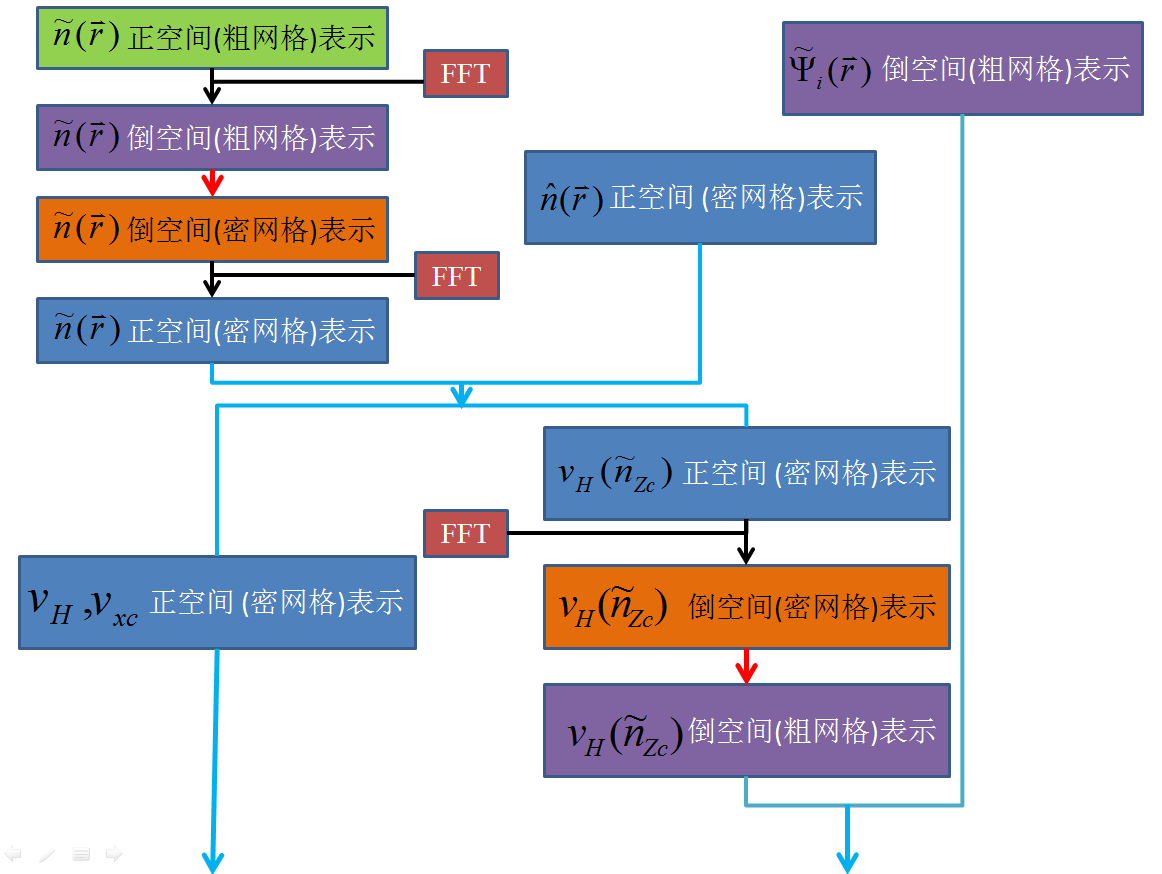
\includegraphics[height=2.7in,width=4.0in,viewport=0 0 1180 875,clip]{Figures/dual_grid.png}
%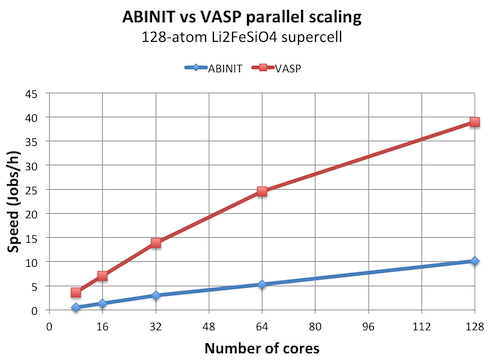
\includegraphics[height=1.50in,width=1.95in,viewport=0 0 240 200,clip]{Figures/VASP-abinit_Li128-2.png}
%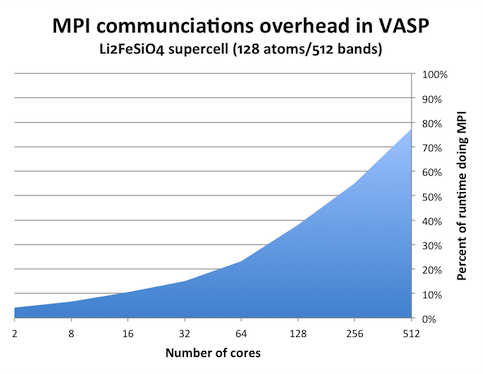
\includegraphics[height=1.50in,width=1.90in,viewport=0 0 240 200,clip]{Figures/VASP-mpi-Li128.png}
%%\caption{\tiny \textrm{The comparison of parallel scaling for ABINIT vs VASP.}}%(与文献\cite{EPJB33-47_2003}图1对比)
%\label{ABINIT_vs_VASP-1}
%\end{figure} 
}

\section{\rm{POTCAR}是\rm{VASP}软件的数据基础}
\frame
{
	\frametitle{\textrm{PAW}方法的核心思想}
\begin{figure}[h!]
\centering
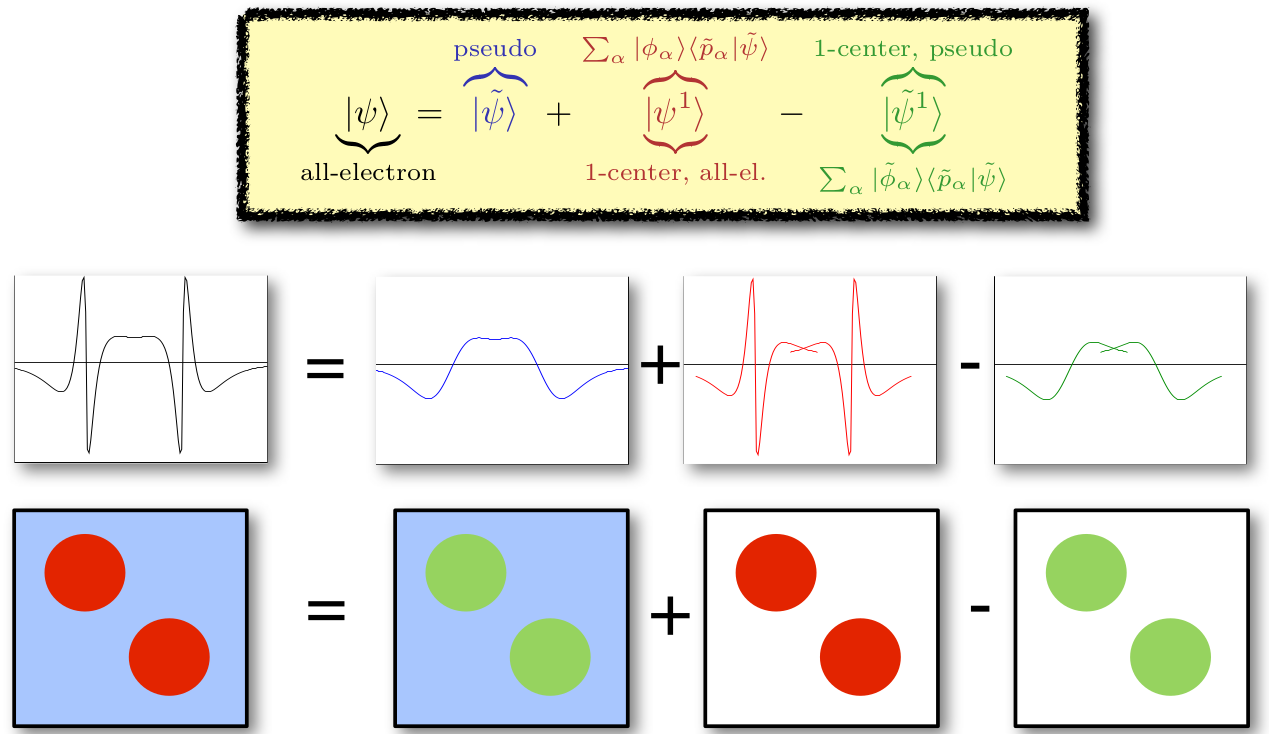
\includegraphics[height=2.3in,width=4.0in,viewport=0 0 1280 745,clip]{Figures/PAW-baseset.png}
\caption{\tiny \textrm{The Augmentation of PAW.}}%(与文献\cite{EPJB33-47_2003}图1对比)
\label{PAW_baseset}
\end{figure}
}

\frame
{
\frametitle{电荷密度的重新分解}
\textrm{PAW}方法提出后有很长一段时间没有能够得到广泛应用\\
\textrm{G. Kresse}等将%\textrm{Bl\"ochl}的
初始方案中电荷密度按价电子-芯电子作了重新划分
\begin{itemize}
	\item 芯层电荷与核电荷构成离子实电荷:~$n_{Zc}=n_Z+n_c$
\begin{figure}[h!]
\centering
\vspace{-10.5pt}
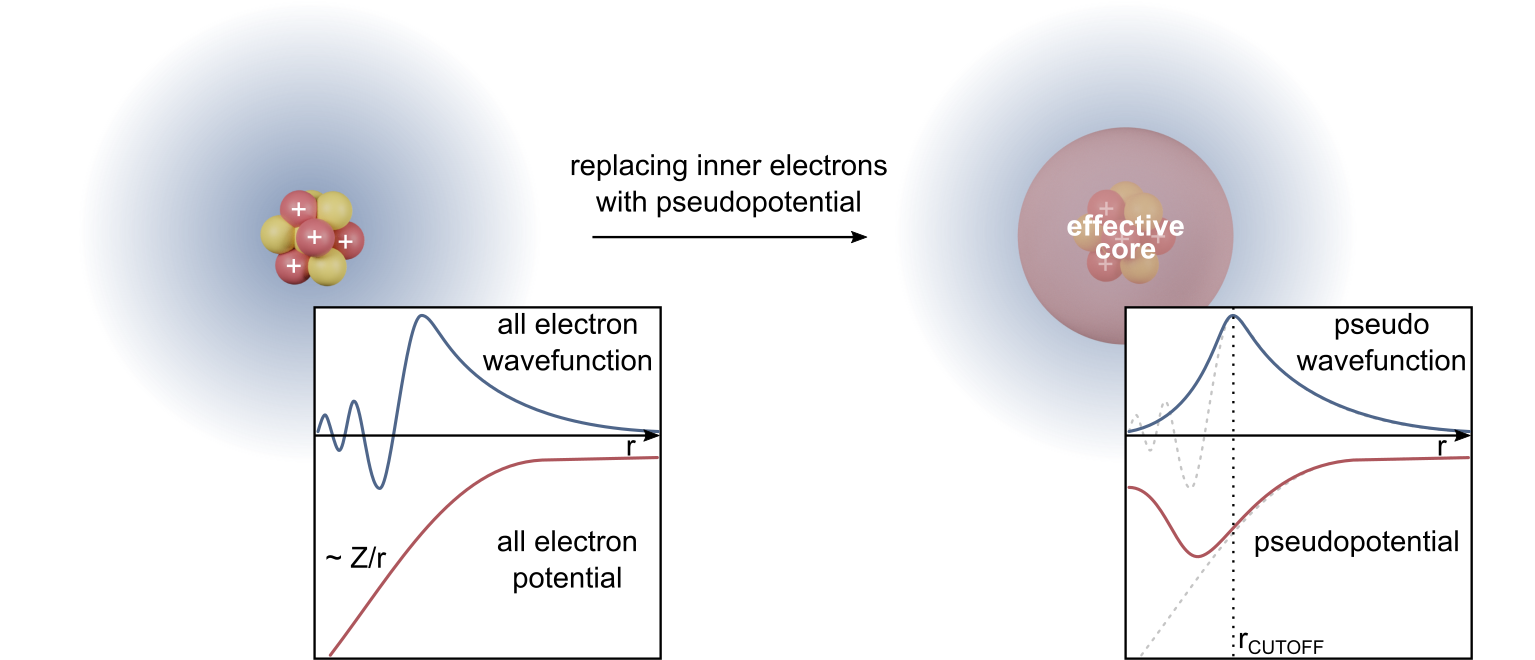
\includegraphics[height=1.4in,width=2.8in,viewport=0 0 380 190,clip]{Figures/Pseudo-potential_charge.png}
\caption{\tiny \textrm{The difference of the electron-density distributing from P. Bl\"ochl  and from G. Kresse.}}%(与文献\cite{EPJB33-47_2003}图1对比)
\label{PAW_Pseudo-Charge}
\end{figure}
	\item \textrm{VASP}的实现方案:~将\textrm{PAW}方法与\textrm{USPP}方法关联起来
\end{itemize}
}

\frame
{
	\frametitle{\rm{VASP}的\rm{POTCAR}文件}
\centering
\vspace{-0.15in}
%------------------------------------直-接-插-入-文-件--------------------------------------------------------------------------------------
%\textcolor{red}{\textbf{直接插入文件}}:
\fontsize{4.8pt}{4.2pt}\selectfont{
%\verbatiminput{/home/jiangjun/Documents/Latex_Beamer/Figures/VASP-POTCAR_Si-00-PSCTR} %为保险:~选用文件名绝对路径
\verbatiminput{Figures/VASP-POTCAR_Si-00-PSCTR} %为保险:~选用文件名绝对路径
}
}

\frame
{
	\frametitle{\textrm{POTCAR}文件:~倒空间局域赝势函数}
\begin{minipage}{0.40\textwidth}
\centering
%\vspace{0.05in}
%------------------------------------直-接-插-入-文-件--------------------------------------------------------------------------------------
%\textcolor{red}{\textbf{直接插入文件}}:
\fontsize{2.7pt}{1.2pt}\selectfont{
%\verbatiminput{/home/jiangjun/Documents/Latex_Beamer/Figures/VASP-POTCAR_Si-01-localpotential-part} %为保险:~选用文件名绝对路径
\verbatiminput{Figures/VASP-POTCAR_Si-01-localpotential-part} %为保险:~选用文件名绝对路径
}
\end{minipage}
\begin{minipage}{0.58\textwidth}
%{\fontsize{5.5pt}{4.2pt}\selectfont{
%	\begin{displaymath}
%		G_{\max}^1
%	\end{displaymath}
%	\begin{displaymath}
%		\begin{aligned}
%			\tilde{V}(q)=&\frac{4\pi}{q}\int\sin(q\cdot r)\tilde{V}(r)\cdot r\mathrm{d}r\\
%			\tilde{V}(q)\cdot q=&4\pi\int_0^{\infty}\sin(q\cdot r)\tilde{V}(r)\cdot r\mathrm{d}r\\
%%			\tilde{V}_{\mathrm{ion}}(q)=&-\frac{4\pi Z_{\mathrm{ion}}(1-\mathrm{e}^{-q^2/4\alpha})}{q^2}\\
%			\tilde{V}(q=0)=&0
%		\end{aligned}
%\end{displaymath} }}
\begin{figure}[t!]
\centering
\vspace{-0.15in}
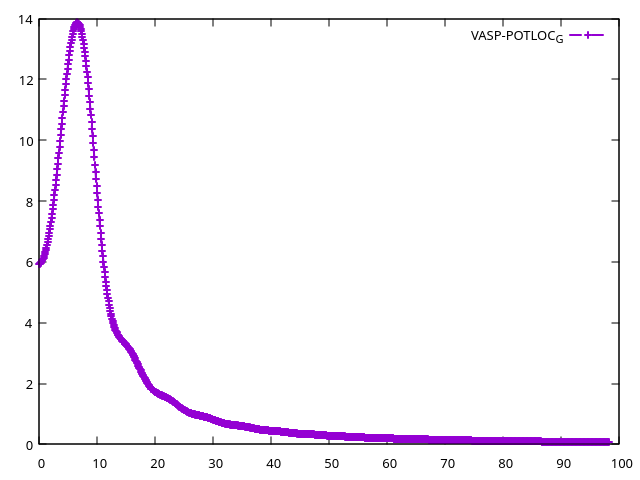
\includegraphics[width=2.3in,height=1.75in,viewport=0 0 500 360, clip]{Figures/VASP_POTLOC_G.png}
\label{local-potential}
\end{figure}
\end{minipage}
}

\frame
{
	\frametitle{\textrm{POTCAR}文件:~倒空间赝芯电荷}
\begin{minipage}{0.40\textwidth}
\centering
\vspace{-0.05in}
%------------------------------------直-接-插-入-文-件--------------------------------------------------------------------------------------
%\textcolor{red}{\textbf{直接插入文件}}:
\fontsize{2.7pt}{1.2pt}\selectfont{
%\verbatiminput{/home/jiangjun/Documents/Latex_Beamer/Figures/VASP-POTCAR_Si-02-localcorecharge} %为保险:~选用文件名绝对路径
\verbatiminput{Figures/VASP-POTCAR_Si-02-localcorecharge} %为保险:~选用文件名绝对路径
}
\end{minipage}
\begin{minipage}{0.58\textwidth}
{\fontsize{7.2pt}{6.2pt}\selectfont{
	\vskip -5.0in
	\begin{displaymath}
		\begin{aligned}
%			\tilde{V}(q)=&\frac{4\pi}{q}\int\sin(q\cdot r)\tilde{V}(r)\cdot r\mathrm{d}r\\
			\tilde{\rho}_{\mathrm{core}}(q)\cdot q=&4\pi\int_0^{\infty}\sin(q\cdot r)\tilde{\rho}_{\mathrm{core}}(r)\cdot r\mathrm{d}r\\
%			=&\frac{4\pi}{q}\int_0^{\infty}\sin(q\cdot r)V(r)\cdot r\mathrm{d}r
		\end{aligned}
\end{displaymath}
}}
\end{minipage}
}

\frame
{
	\frametitle{\textrm{POTCAR}文件:~赝电荷密度}
\begin{minipage}{0.40\textwidth}
\centering
\vspace{-0.05in}
%------------------------------------直-接-插-入-文-件--------------------------------------------------------------------------------------
%\textcolor{red}{\textbf{直接插入文件}}:
\fontsize{2.7pt}{1.2pt}\selectfont{
%\verbatiminput{/home/jiangjun/Documents/Latex_Beamer/Figures/VASP-POTCAR_Si-03-pseudo-charge} %为保险:~选用文件名绝对路径
\verbatiminput{Figures/VASP-POTCAR_Si-03-pseudo-charge} %为保险:~选用文件名绝对路径
}
\end{minipage}
\begin{minipage}{0.58\textwidth}
{\fontsize{7.2pt}{6.2pt}\selectfont{
	\vskip -5.0in
	\begin{displaymath}
		\tilde{\rho}(q)=\frac{\tilde{V}(q)}{4\pi}\cdot q^2
\end{displaymath}
}}
\end{minipage}
}

\frame
{
	\frametitle{\textrm{POTCAR}文件:~投影函数}
\begin{minipage}{0.58\textwidth}
\centering
\vspace{-0.05in}
%------------------------------------直-接-插-入-文-件--------------------------------------------------------------------------------------
%\textcolor{red}{\textbf{直接插入文件}}:
\fontsize{2.6pt}{1.2pt}\selectfont{
%\verbatiminput{/home/jiangjun/Documents/Latex_Beamer/Figures/VASP-POTCAR_Si-04-projector-1} %为保险:~选用文件名绝对路径
\verbatiminput{Figures/VASP-POTCAR_Si-04-projector-1} %为保险:~选用文件名绝对路径
}
\end{minipage}
\hfill
\begin{minipage}{0.40\textwidth}
{\fontsize{5.5pt}{4.2pt}\selectfont{
%	\begin{displaymath}
%		\begin{aligned}
%			& G_{\max}^2 \\
%			& r_{\max,0}^{\mathrm{pro}}
%		\end{aligned}
%	\end{displaymath}
%	\vskip 10pt
	\begin{displaymath}
		\begin{aligned}
%			\hat{T}|\psi_i\rangle=&\left[-\nabla^2-\frac{l(l+1)}2\right]|\psi_i\rangle\\
			D_{ij}^{\mathrm{ion}}=&\langle\psi_i|\hat{T}+V_{\mathrm{eff}}|\psi_j\rangle\\
			-&\langle\tilde{\psi}_i|\hat{T}+\tilde{V}_{\mathrm{eff}}|\tilde{\psi}_j\rangle\\
			-&\int\hat{Q}_{ij}^{00}(r)\tilde{V}(r)\mathrm{d}r
		\end{aligned}
	\end{displaymath}
%	\vskip 70pt
\begin{figure}[t!]
\centering
\vspace{-0.15in}
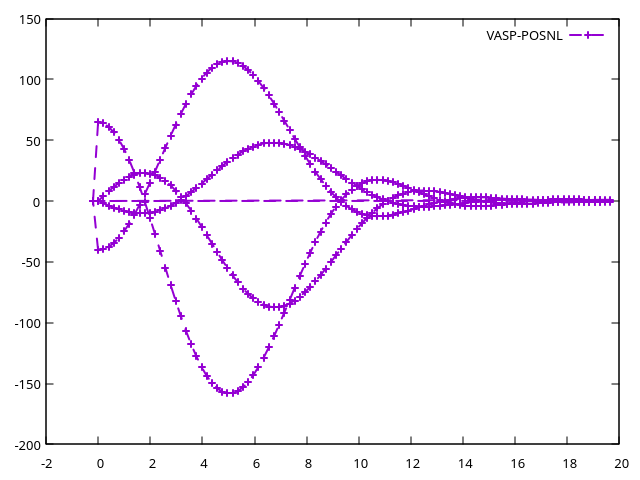
\includegraphics[width=1.3in,height=0.75in,viewport=0 0 500 360, clip]{Figures/VASP-project.png}
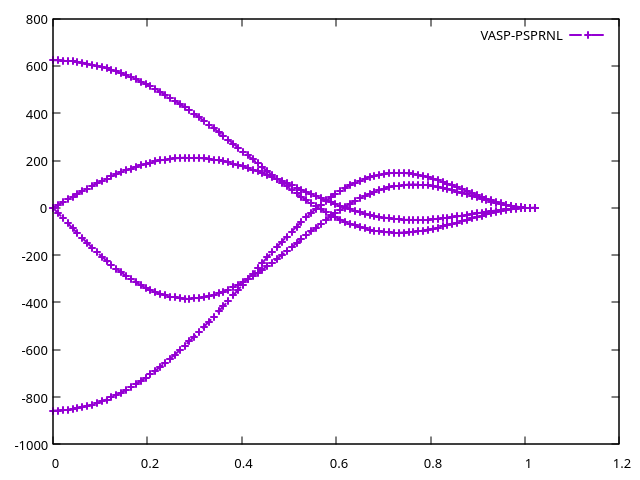
\includegraphics[width=1.3in,height=0.75in,viewport=0 0 500 360, clip]{Figures/VASP-project-R.png}
\label{PROJECTOR}
\end{figure}
	\begin{displaymath}
		\langle\tilde{p}_i|\tilde\phi_j\rangle=\delta_{ij}	
	\end{displaymath}}}
\end{minipage}
}

%\frame
%{
%	\frametitle{\textrm{POTCAR}文件}
%\centering
%\vspace{-0.15in}
%%------------------------------------直-接-插-入-文-件--------------------------------------------------------------------------------------
%%\textcolor{red}{\textbf{直接插入文件}}:
%\fontsize{2.6pt}{1.2pt}\selectfont{
%%\verbatiminput{/home/jiangjun/Documents/Latex_Beamer/Figures/VASP-POTCAR_Si-04-projector-2} %为保险:~选用文件名绝对路径
%\verbatiminput{Figures/VASP-POTCAR_Si-04-projector-2} %为保险:~选用文件名绝对路径
%}
%}

\frame
{
	\frametitle{\textrm{POTCAR}文件:~补偿电荷}
\centering
\vspace{-0.15in}
%------------------------------------直-接-插-入-文-件--------------------------------------------------------------------------------------
%\textcolor{red}{\textbf{直接插入文件}}:
\fontsize{4.8pt}{4.2pt}\selectfont{
%\verbatiminput{/home/jiangjun/Documents/Latex_Beamer/Figures/VASP-POTCAR_Si-05-augmentcharge} %为保险:~选用文件名绝对路径
\verbatiminput{Figures/VASP-POTCAR_Si-05-augmentcharge} %为保险:~选用文件名绝对路径
}
\begin{displaymath}
	\langle\phi_i|\phi_i\rangle-\langle\tilde\phi|\tilde\phi_i\rangle
\end{displaymath}
}

\frame
{
	\frametitle{\textrm{POTCAR}文件:~径向对数布点}
\begin{minipage}{0.58\textwidth}
\centering
\vspace{-0.05in}
%------------------------------------直-接-插-入-文-件--------------------------------------------------------------------------------------
%\textcolor{red}{\textbf{直接插入文件}}:
\fontsize{3.3pt}{1.9pt}\selectfont{
%\verbatiminput{/home/jiangjun/Documents/Latex_Beamer/Figures/VASP-POTCAR_Si-06-grid} %为保险:~选用文件名绝对路径
\verbatiminput{Figures/VASP-POTCAR_Si-06-grid} %为保险:~选用文件名绝对路径
}
\end{minipage}
\hfill
\begin{minipage}{0.40\textwidth}
{\fontsize{8.2pt}{6.2pt}\selectfont{
	\centering{径向部分的对数布点:}
	\begin{displaymath}
		r(i)=r(1)*10^{(i-1)\cdot\Delta h}
	\end{displaymath}}}
\end{minipage}
}

\frame
{
	\frametitle{\textrm{POTCAR}文件:~原子芯电荷势}
\begin{minipage}{0.58\textwidth}
\centering
\vspace{-0.05in}
%------------------------------------直-接-插-入-文-件--------------------------------------------------------------------------------------
%\textcolor{red}{\textbf{直接插入文件}}:
\fontsize{3.3pt}{1.9pt}\selectfont{
%\verbatiminput{/home/jiangjun/Documents/Latex_Beamer/Figures/VASP-POTCAR_Si-07-aepotential} %为保险:~选用文件名绝对路径
\verbatiminput{Figures/VASP-POTCAR_Si-07-aepotential} %为保险:~选用文件名绝对路径
}
\end{minipage}
\hfill
\begin{minipage}{0.40\textwidth}
\begin{figure}[t!]
\centering
\vspace{-0.15in}
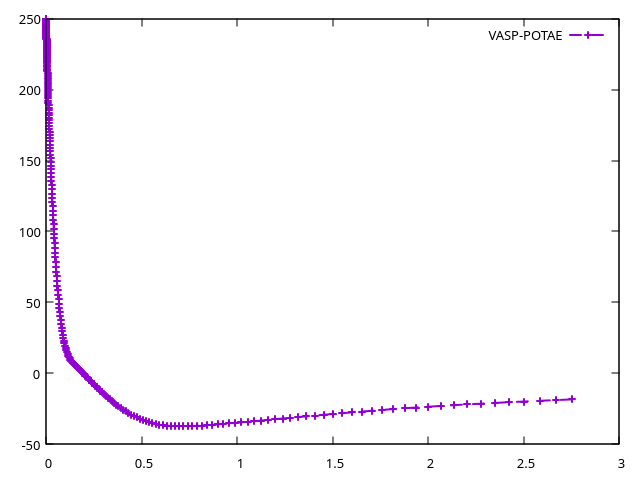
\includegraphics[width=1.8in,height=1.05in,viewport=0 0 500 360, clip]{Figures/VASP_POTAE.png}
\label{VASP_POTAE}
\end{figure}
\end{minipage}
}

\frame
{
	\frametitle{\textrm{POTCAR}文件:~芯电荷密度}
\begin{minipage}{0.58\textwidth}
\centering
\vspace{-0.05in}
%------------------------------------直-接-插-入-文-件--------------------------------------------------------------------------------------
%\textcolor{red}{\textbf{直接插入文件}}:
\fontsize{3.3pt}{1.9pt}\selectfont{
%\verbatiminput{/home/jiangjun/Documents/Latex_Beamer/Figures/VASP-POTCAR_Si-08-corecharge} %为保险:~选用文件名绝对路径
\verbatiminput{Figures/VASP-POTCAR_Si-08-corecharge} %为保险:~选用文件名绝对路径
}
\end{minipage}
\hfill
\begin{minipage}{0.40\textwidth}
\begin{figure}[t!]
\centering
\vspace{-0.15in}
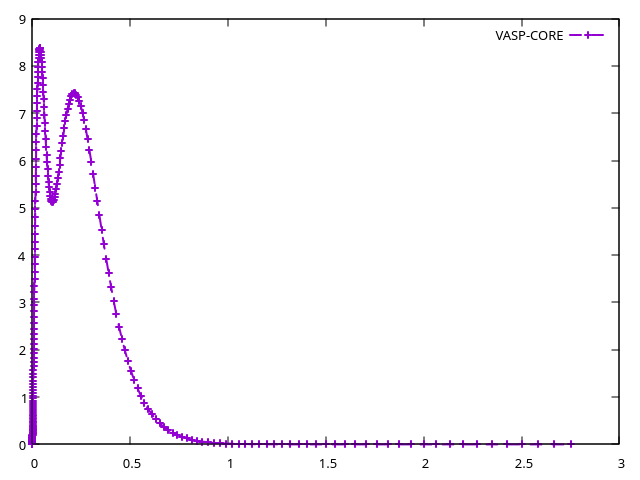
\includegraphics[width=1.8in,height=1.05in,viewport=0 0 500 360, clip]{Figures/VASP-CORE.png}
\label{VASP_POTCORE}
\end{figure}
\end{minipage}
}

\frame
{
	\frametitle{\textrm{POTCAR}文件:~动能密度}
\begin{minipage}{0.58\textwidth}
\centering
\vspace{-0.05in}
%------------------------------------直-接-插-入-文-件--------------------------------------------------------------------------------------
%\textcolor{red}{\textbf{直接插入文件}}:
\fontsize{3.3pt}{1.9pt}\selectfont{
%\verbatiminput{/home/jiangjun/Documents/Latex_Beamer/Figures/VASP-POTCAR_Si-09-kinetic-ene-den} %为保险:~选用文件名绝对路径
\verbatiminput{Figures/VASP-POTCAR_Si-09-kinetic-ene-den} %为保险:~选用文件名绝对路径
}
\end{minipage}
\hskip 2pt
\begin{minipage}{0.40\textwidth}
{\fontsize{5.5pt}{4.2pt}\selectfont{
	\begin{displaymath}
		\hspace*{5pt}	\langle\phi_i|\hat{T}|\phi_i\rangle=\langle\phi_j|\left[-\nabla^2-\frac{l(l+1)}2\right]|\phi_i\rangle
\end{displaymath}}}
\end{minipage}
}

\frame
{
	\frametitle{\textrm{POTCAR}文件:~赝局域势}
\begin{minipage}{0.58\textwidth}
\centering
\vspace{-0.10in}
%------------------------------------直-接-插-入-文-件--------------------------------------------------------------------------------------
%\textcolor{red}{\textbf{直接插入文件}}:
\fontsize{3.3pt}{1.9pt}\selectfont{
%\verbatiminput{/home/jiangjun/Documents/Latex_Beamer/Figures/VASP-POTCAR_Si-10-pspotential} %为保险:~选用文件名绝对路径
\verbatiminput{Figures/VASP-POTCAR_Si-10-pspotential} %为保险:~选用文件名绝对路径
}
\end{minipage}
\hskip 2pt
\begin{minipage}{0.40\textwidth}
\begin{figure}[t!]
\centering
\vspace{-0.15in}
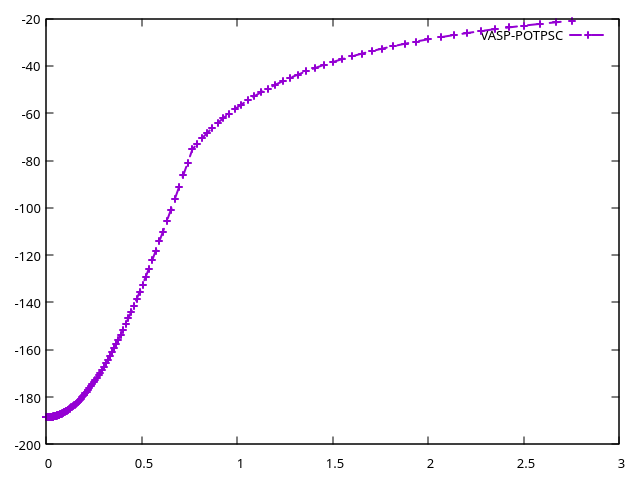
\includegraphics[width=1.8in,height=1.05in,viewport=0 0 500 360, clip]{Figures/VASP_POTPSC.png}
\label{VASP_POTPSC}
\end{figure}
\end{minipage}
}

\frame
{
	\frametitle{\textrm{POTCAR}文件:~赝芯电荷}
\begin{minipage}{0.58\textwidth}
\centering
\vspace{-0.10in}
%------------------------------------直-接-插-入-文-件--------------------------------------------------------------------------------------
%\textcolor{red}{\textbf{直接插入文件}}:
\fontsize{3.3pt}{1.9pt}\selectfont{
%\verbatiminput{/home/jiangjun/Documents/Latex_Beamer/Figures/VASP-POTCAR_Si-11-pscoreden} %为保险:~选用文件名绝对路径
\verbatiminput{Figures/VASP-POTCAR_Si-11-pscoreden} %为保险:~选用文件名绝对路径
}
\end{minipage}
\hfill
\begin{minipage}{0.40\textwidth}
\begin{figure}[t!]
\centering
\vspace{-0.15in}
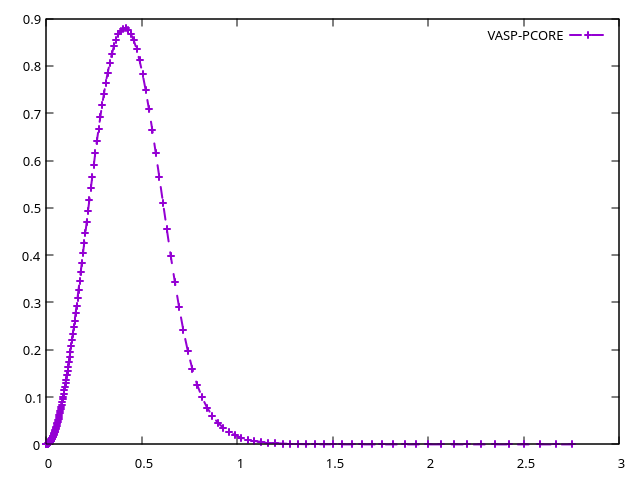
\includegraphics[width=1.8in,height=1.05in,viewport=0 0 500 360, clip]{Figures/VASP_PCORE.png}
\label{VASP_PCORE}
\end{figure}
\end{minipage}
}

\frame
{
	\frametitle{\textrm{POTCAR}文件:~赝波函数}
\begin{minipage}{0.58\textwidth}
\centering
\vspace{-0.15in}
%------------------------------------直-接-插-入-文-件--------------------------------------------------------------------------------------
%\textcolor{red}{\textbf{直接插入文件}}:
\fontsize{3.3pt}{1.9pt}\selectfont{
%\verbatiminput{/home/jiangjun/Documents/Latex_Beamer/Figures/VASP-POTCAR_Si-12-pswav-4} %为保险:~选用文件名绝对路径
\verbatiminput{Figures/VASP-POTCAR_Si-12-pswav-4} %为保险:~选用文件名绝对路径
}
\end{minipage}
\hfill
\begin{minipage}{0.40\textwidth}
\begin{figure}[t!]
\centering
\vspace{-0.15in}
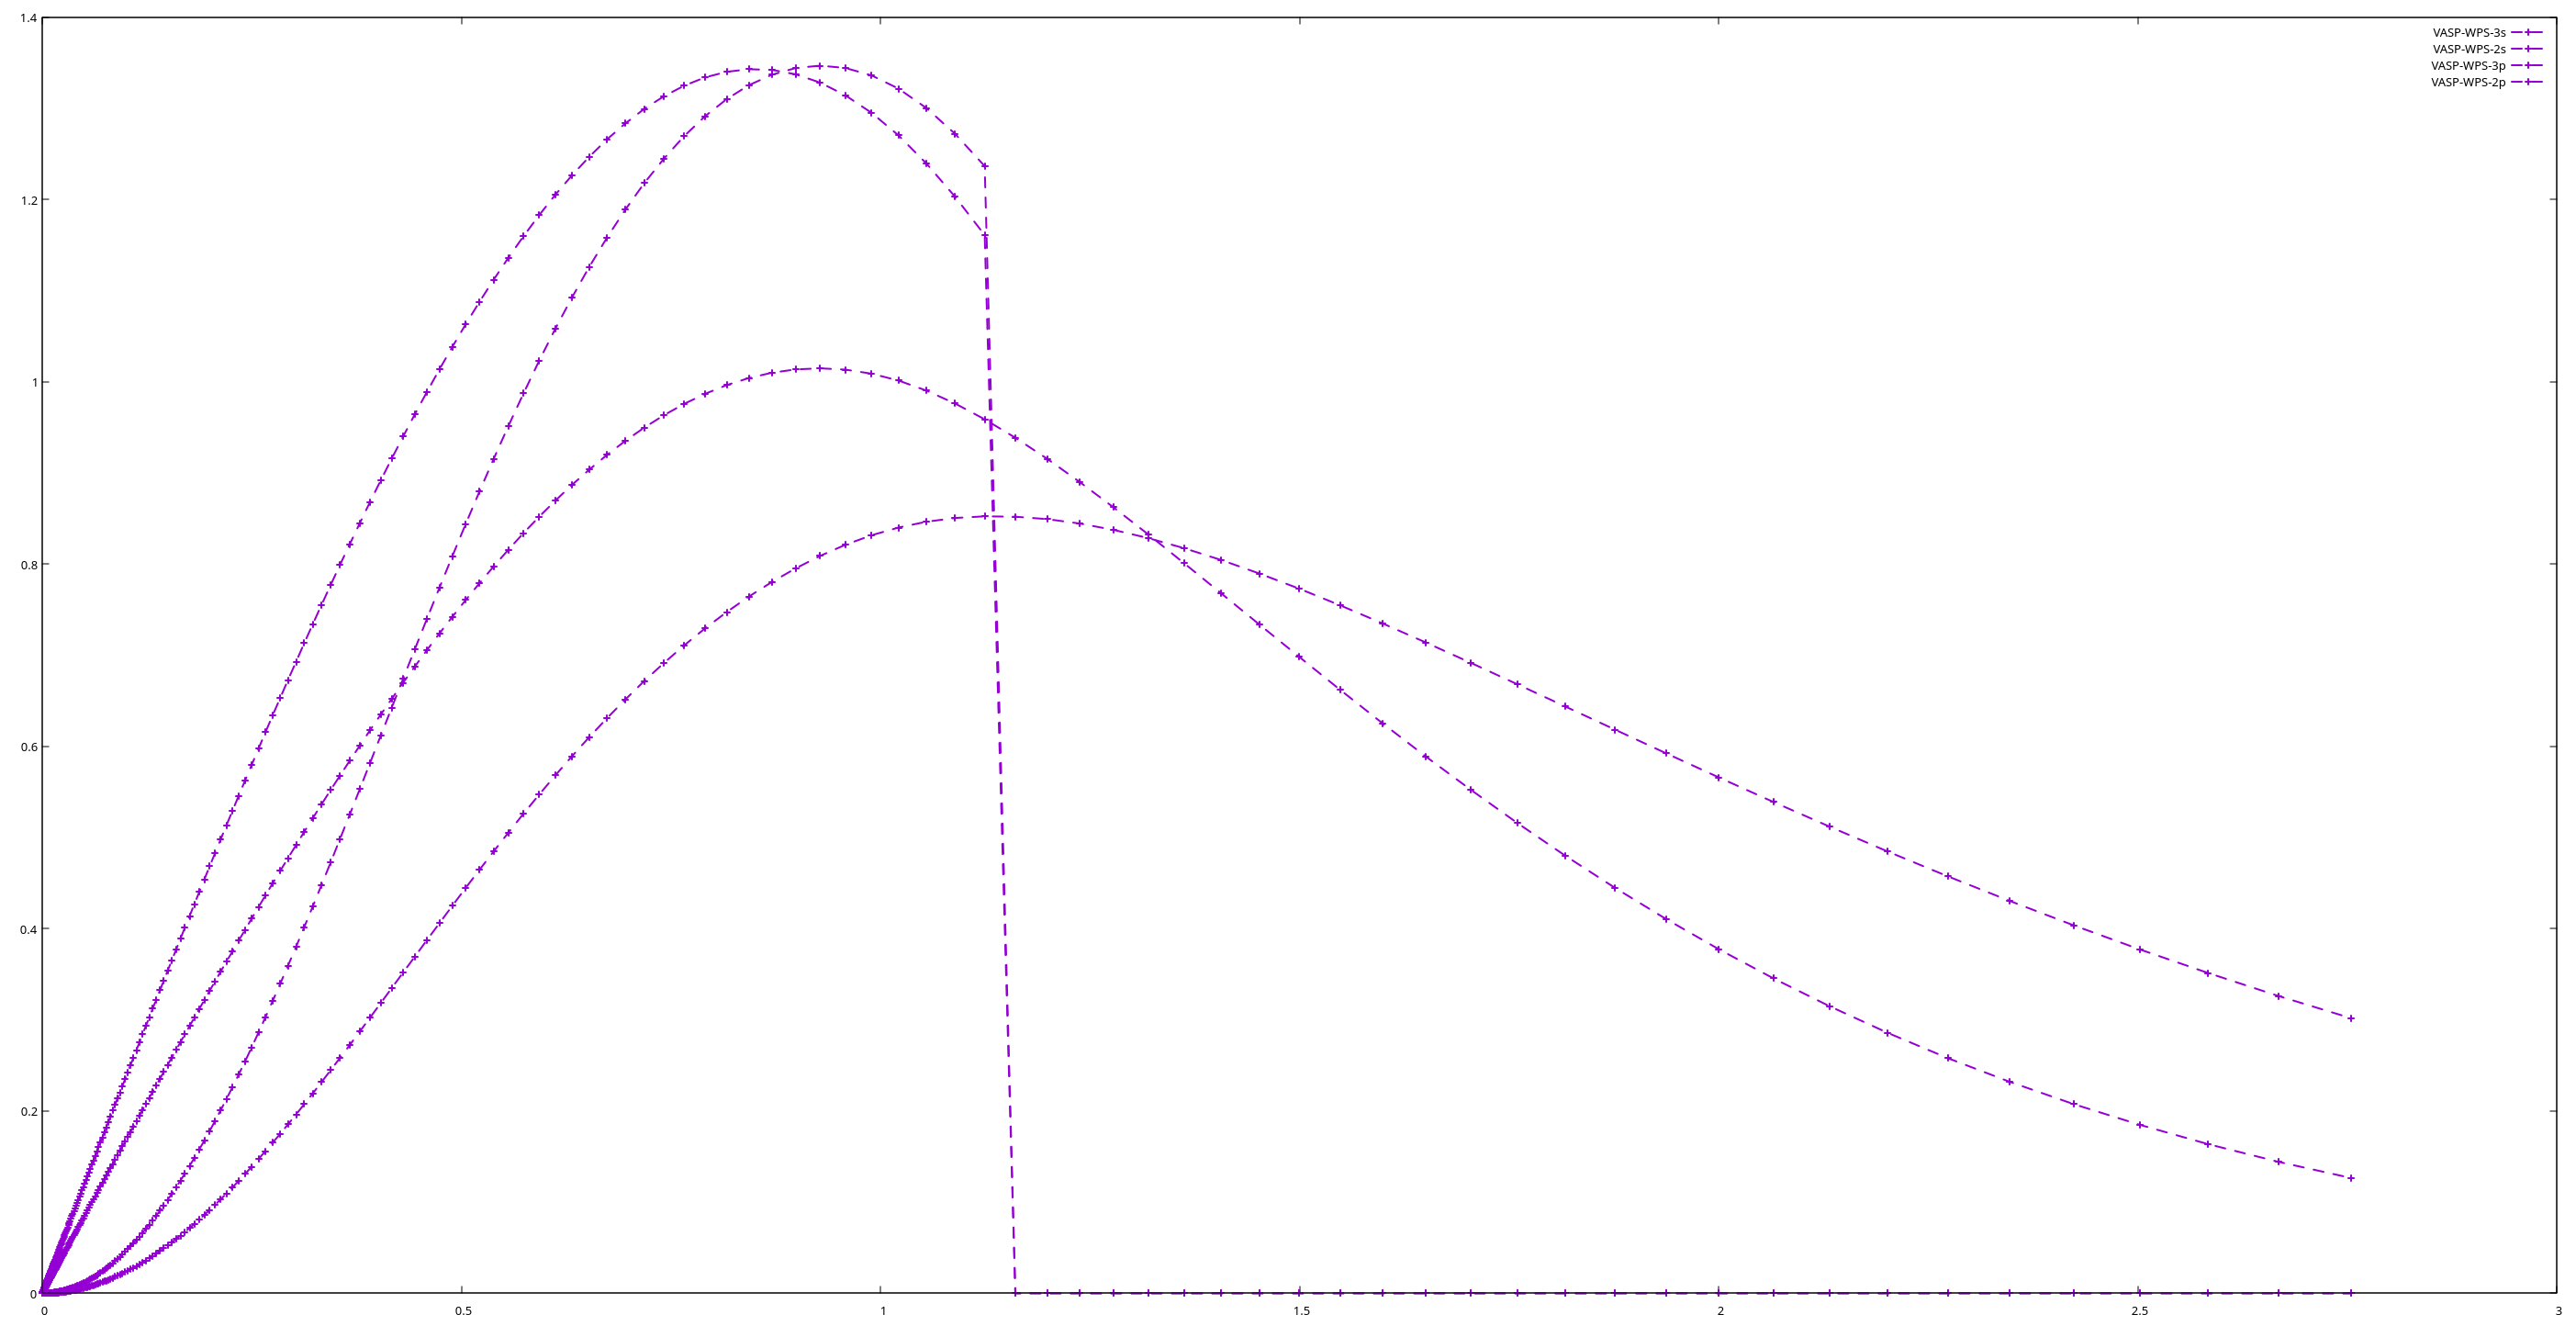
\includegraphics[width=1.8in,height=1.05in,viewport=0 0 2200 1160, clip]{Figures/VASP_WPS.png}
\label{VASP_WPS}
\end{figure}
\end{minipage}
}

\frame
{
	\frametitle{\textrm{POTCAR}文件:~全电子波函数}
\begin{minipage}{0.58\textwidth}
\centering
\vspace{-0.15in}
%------------------------------------直-接-插-入-文-件--------------------------------------------------------------------------------------
%\textcolor{red}{\textbf{直接插入文件}}:
\fontsize{3.3pt}{1.9pt}\selectfont{
%\verbatiminput{/home/jiangjun/Documents/Latex_Beamer/Figures/VASP-POTCAR_Si-12-aewav-4} %为保险:~选用文件名绝对路径
\verbatiminput{Figures/VASP-POTCAR_Si-12-aewav-4} %为保险:~选用文件名绝对路径
}
\end{minipage}
\hfill
\begin{minipage}{0.40\textwidth}
\begin{figure}[t!]
\centering
\vspace{-0.15in}
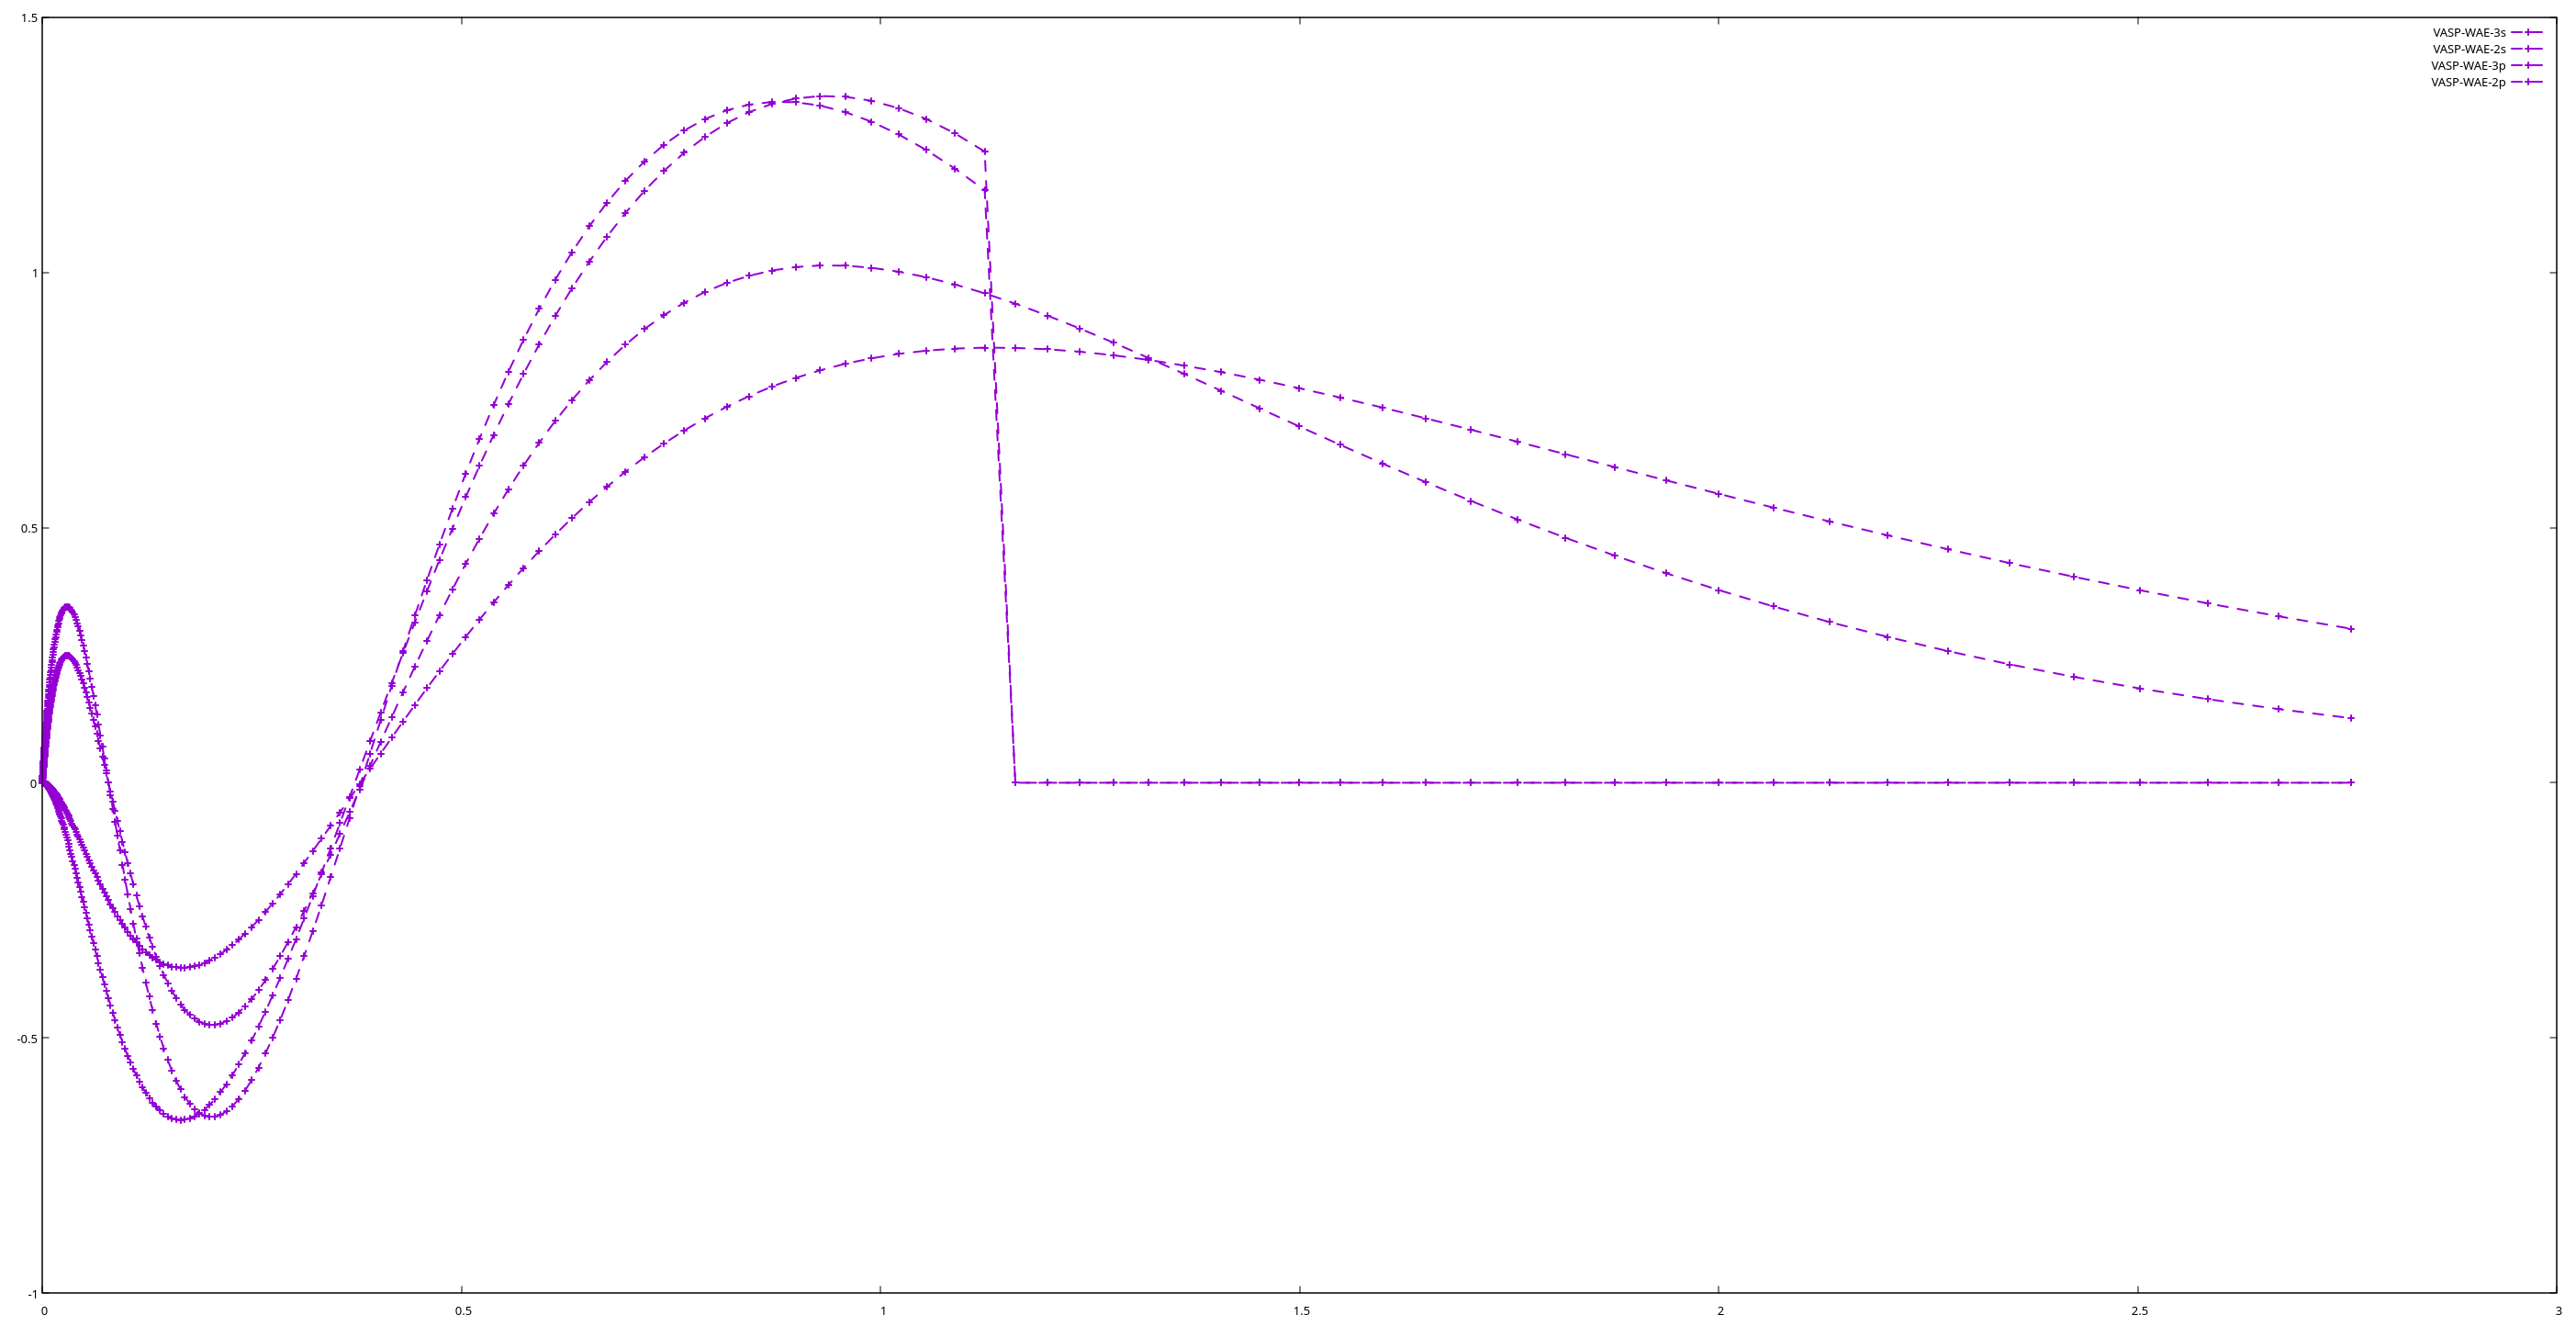
\includegraphics[width=1.8in,height=1.05in,viewport=0 0 2200 1160, clip]{Figures/VASP_WAE.png}
\label{VASP_WAE}
\end{figure}
\end{minipage}
}

\frame
{
	\frametitle{\textrm{VASP}计算中的原子数据}
	\textrm{POTCAR}是\textrm{VASP}的必要文件，提供了\textrm{VASP}计算所需的全部原子数据，也是\textrm{VASP}完成\textrm{PAW}方法的主要基础
	\begin{itemize}
		\item \textrm{POTCAR}是\textrm{VASP}实现材料精确计算的重要保证\\
			同样都应用\textrm{PAW}方法，\textcolor{blue}{公认\textrm{VASP}较\textrm{QE}、\textrm{ABINIT}等软件的计算精度要高}
		\item \textrm{POTCAR}数据 生成依赖较多的可调参数\\
			包括能量参数$\varepsilon_l$、多种截断半径$r_c$、$r_{\mathrm{vloc}}$、$r_{\mathrm{shape}}$、$r_{\mathrm{core}}$
		\item \textcolor{red}{\textrm{POTCAR}数据生成代码是\textrm{VASP}中唯一没有公开的}
		\item 用\textrm{VASP}模拟极端条件下材料物性的能力，受到\textrm{POTCAR}数据的制约
	\end{itemize}
	%文献\cite{PRB59-1758_1999}介绍了\textrm{POTCAR}的主要实现思想

%当前研究主要尝试:~
	基于开源的\textrm{PAW}原子数据生成软件(\textrm{atomPAW})，开发生成\textrm{POTCAR}原子数据的功能
}

\section{\rm{VASP}的原子数据重建}
\frame
{
	\frametitle{\textrm{PAW}原子数据集:~\textrm{wave~function}}
	平滑赝原子分波函数
	\begin{displaymath}
		\tilde\phi_{i=Lk}(\vec r)=Y_L(\widehat{\vec r-\vec R})\tilde\phi_{lk}(|\vec r-\vec R|)
	\end{displaymath}
	\vskip -3pt
	\begin{itemize}
		\item \textrm{Vanderbilt}赝分波函数构建
			\begin{displaymath}
		\tilde\phi_{lk}(r)=\left\{
			\begin{aligned}
				&r^{l+1}\sum_{m=0}^4C_mr^{2m}\quad &r\leqslant r_c^l\\
			&\phi_{lk}(r)\quad&r>r_c^l
			\end{aligned}
		\right.
			\end{displaymath}
			{\fontsize{7.5pt}{5.2pt}\selectfont{系数$C_m$由赝分波函数$\tilde\phi_{lk}(r)$在截断半径$r_c^l$临近5点平滑连续确定}}
		\item \textrm{RRKJ}赝分波函数构建:~由球\textrm{Bessel}函数线性组合%\upcite{JPCM6-8245_1994}
	\begin{displaymath}
		\tilde\phi_{lk}(r)=\left\{
		\begin{aligned} 
			&\sum_{i=1}^2\alpha_ij_l(q_ir)\quad &r\leqslant r_c^l\\
			&\phi_{lk}(r)\quad&r>r_c^l
		\end{aligned}
		\right.
	\end{displaymath}
	{\fontsize{7.5pt}{5.2pt}\selectfont{调节系数$\alpha_i$和$q_i$赝分波函数$\tilde\phi_{lk}(r)$在截断半径$r_c^l$处两阶连续可微}}
%	投影子波函数$\tilde p_i$由\textrm{Gram-Schmidt}正交条件$\langle\tilde p_i|\tilde\phi_j\rangle=\delta_{ij}$确定
	\end{itemize}
}

\frame
{
	\frametitle{\textrm{PAW}原子数据集:~\textrm{wave~function}}
\begin{figure}[h!]
\centering
\vskip -0.5in
\includegraphics[width=1.5in,height=2.7in,viewport=0 0 350 550, angle=-90, clip]{Figures/WAE-data.eps}
\vskip -0.4in
\includegraphics[height=2.7in,width=1.5in,viewport=0 0 350 550, angle=-90, clip]{Figures/WPS-data.eps}
\vskip -0.2in
\caption{\tiny \textrm{The partial wave function.}}%(与文献\cite{EPJB33-47_2003}图1对比)
\label{Wave_Function}
\end{figure}
依据文献的解析形式的确定赝分波函数，对能量参数$\varepsilon_l$、截断半径$r_c^l$包括径向步长的依赖都比较敏感
}

\frame
{
	\frametitle{\textrm{PAW}原子数据集:~\textrm{core~density}}
	赝芯电荷密度$\tilde n_c$构造:%~在截断半径$r_{\mathrm{core}}$内的定义为
	$$\sum_{i=1,2}B_i\dfrac{\sin(q_ir)}r\quad r<r_{\mathrm{core}}$$
	{\fontsize{7.5pt}{5.2pt}\selectfont{调节系数$q_i$和$B_i$使得赝芯电荷密度$\tilde n_c(r)$在截断半径$r_{\mathrm{core}}$处的两阶导数连续}}
\begin{figure}[h!]
\vskip -0.5in
\centering
\hspace*{-0.1in}
\includegraphics[width=1.5in,height=2.35in,viewport=0 0 350 550, angle=-90, clip]{Figures/CORE-data.eps}
\hspace*{-0.7in}
\includegraphics[height=2.35in,width=1.5in,viewport=0 0 350 550, angle=-90, clip]{Figures/PCORE-data.eps}
\caption{\tiny \textrm{The core density.}}%(与文献\cite{EPJB33-47_2003}图1对比)
\label{core_density_Function}
\end{figure}
}

\frame
{
	\frametitle{\textrm{PAW}原子数据集:~$\mathrm{v}_{e\!f\!f}(r)$与$\tilde{\mathrm{v}}_{e\!f\!f}(r)$}
	\textcolor{blue}{原子局域有效势$\mathrm{v}_{e\!f\!f}^a$}
\begin{figure}[h!]
%\vskip -0.5in
\vskip -0.17in
\centering
%\includegraphics[width=1.6in,height=2.7in,viewport=0 0 300 460, angle=-90, clip]{Figures/POTAE-data.eps}
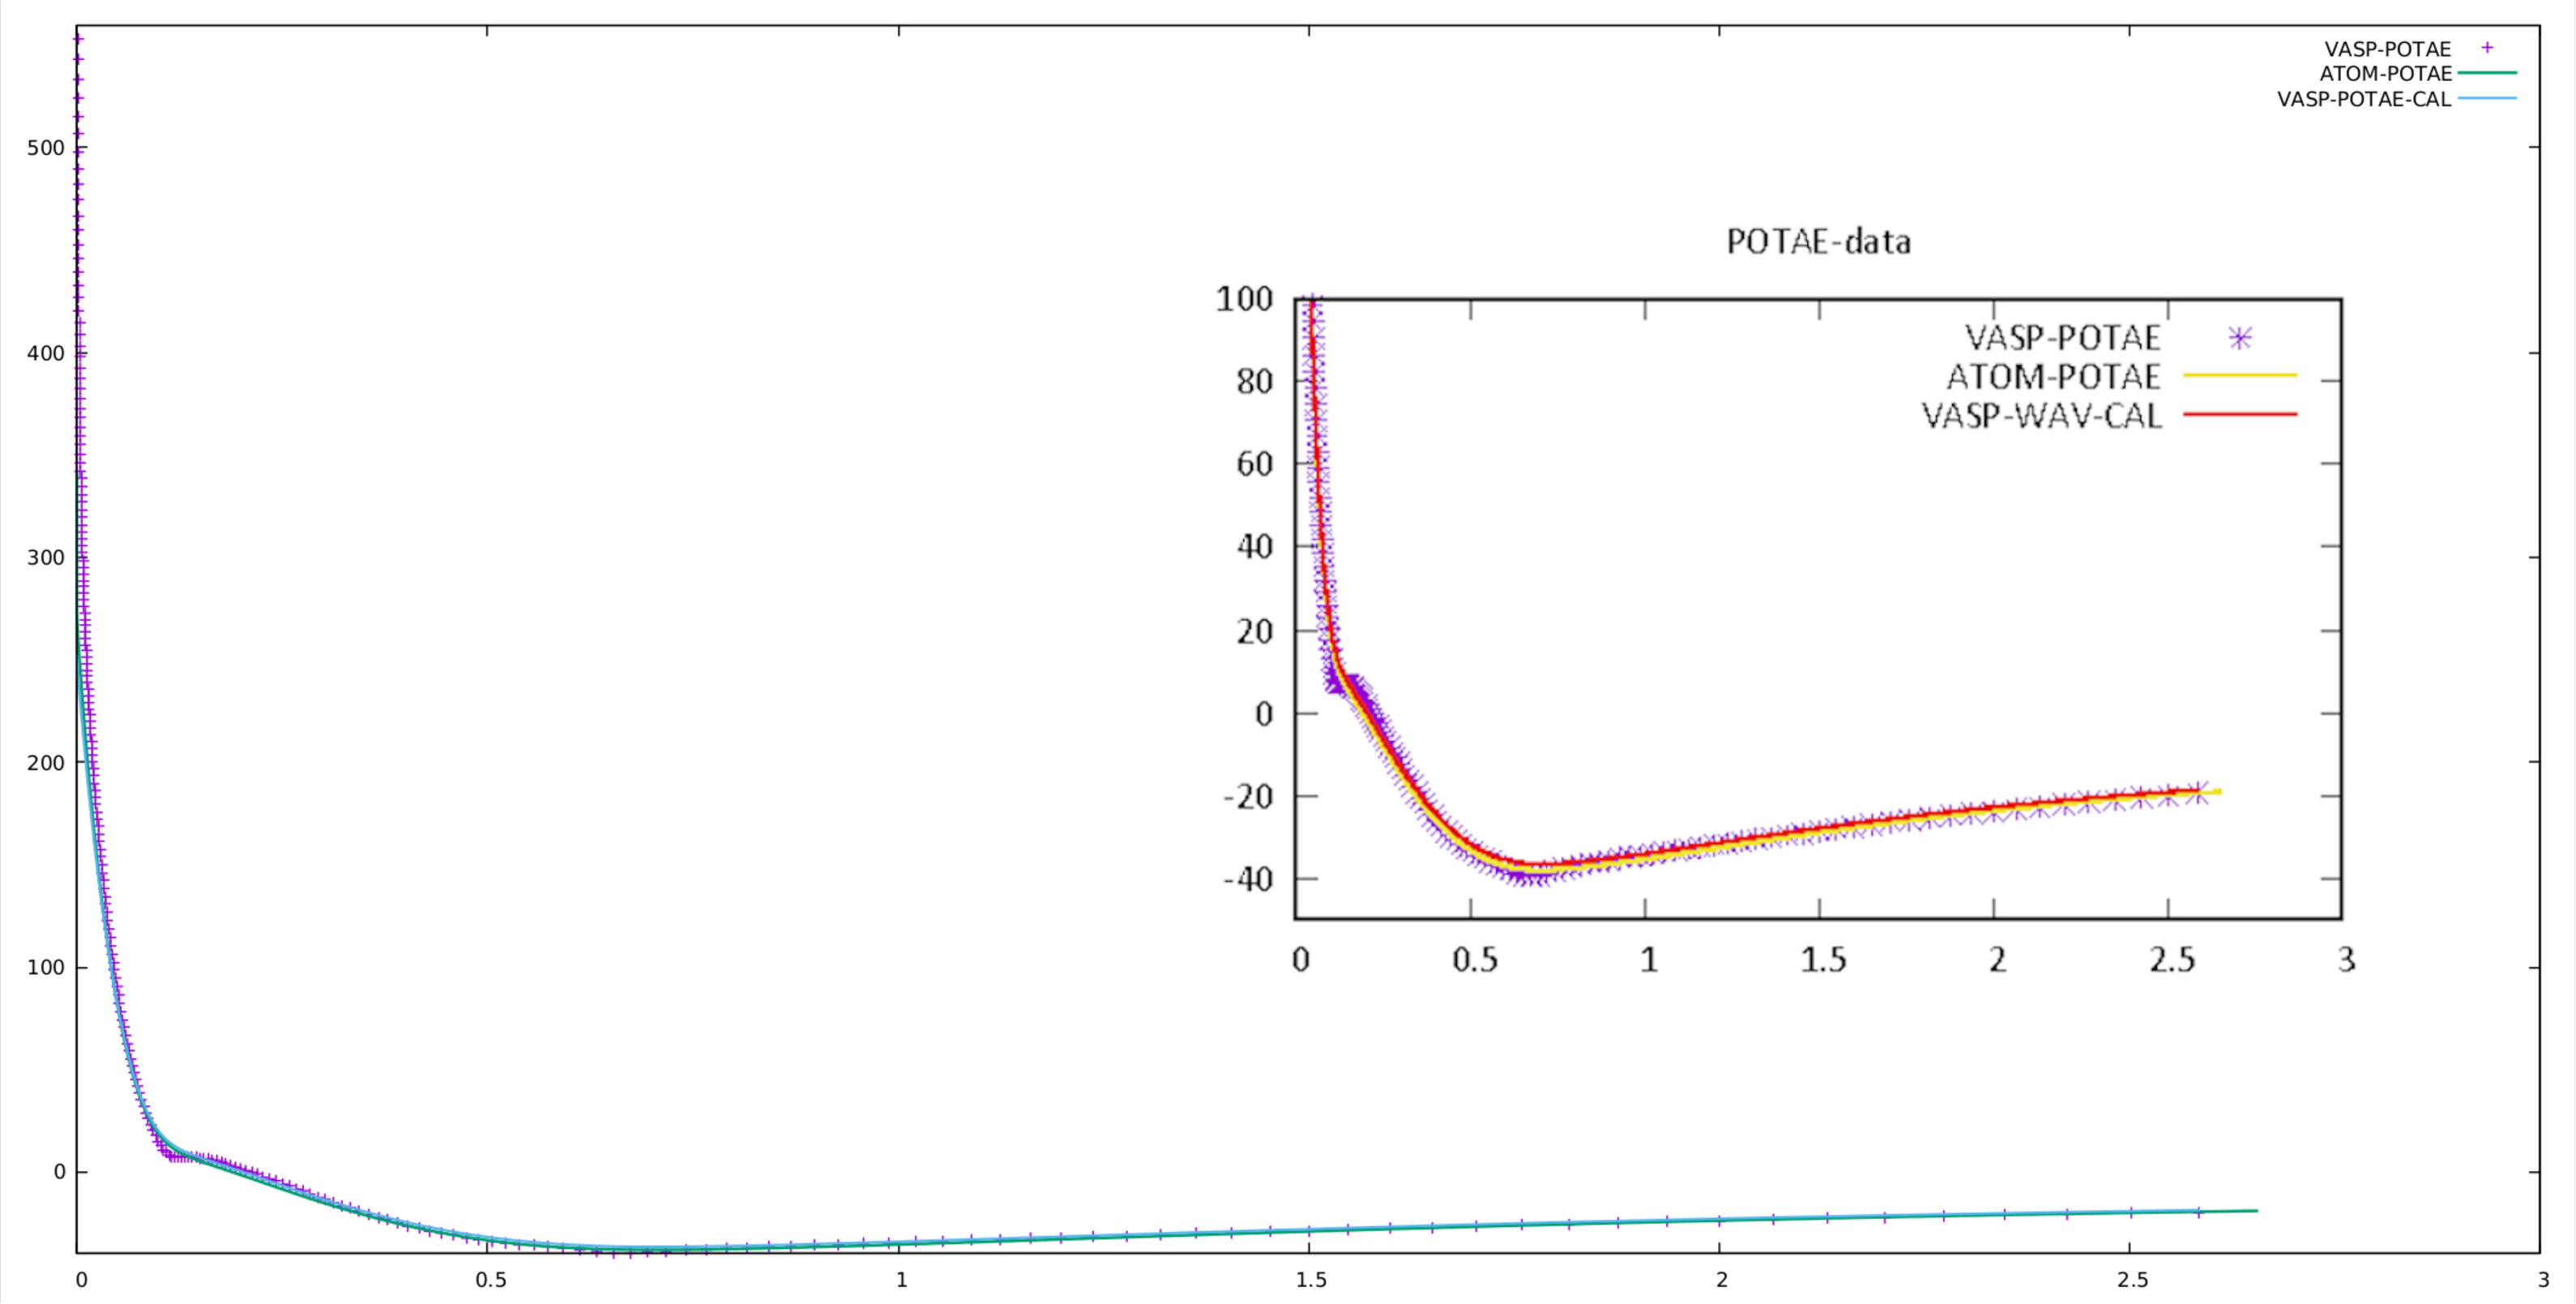
\includegraphics[width=2.5in,height=1.2in,viewport=0 0 1600 800, clip]{Figures/POTAE-full-dat.pdf}
\caption{\tiny \textrm{The local atomic effective-Potential.}}%(与文献\cite{EPJB33-47_2003}图1对比)
\label{local_atomic_PP}
\end{figure}
	\textcolor{blue}{构造原子局域赝势$\tilde v_{e\!f\!f}^a$}%(\textcolor{red}{为防止\textrm{ghost band}})
	:%\\
	(在截断半径$r_{\mathrm{loc}}$内的定义)
	$$\tilde v_{e\!f\!f}^a=A\dfrac{\sin(q_{loc}r)}r\quad r<r_{\mathrm{loc}}$$
	其中$q_{loc}$和$A$要求局域赝势在截断半径$r_{\mathrm{loc}}$处连续到一阶导数
}

\frame
{
	\frametitle{\textrm{PAW}原子数据集:~$\mathrm{v}_H[\tilde n_{Zc}]$}
	局域离子赝势$v_H[\tilde n_{Zc}]$可由原子局域赝势去屏蔽得到
	$$v_H[\tilde n_{Zc}]=\tilde v_{e\!f\!f}^a-v_H[\tilde n_a^1+\hat n_a]-v_{\mathrm{XC}}[\tilde n_a^1+\hat n_a+\tilde n_c]$$
\begin{figure}[h!]
\vskip -0.5in
\centering
\hspace*{-0.1in}
\includegraphics[width=1.5in,height=2.35in,viewport=0 0 350 550, angle=-90, clip]{Figures/POTPS-data.eps}
\hspace*{-0.7in}
\includegraphics[height=2.35in,width=1.5in,viewport=0 0 350 550, angle=-90, clip]{Figures/POTPSC-data.eps}
\caption{\tiny \textrm{The pseudo-potential and local ionic pseudo-potential.}}%(与文献\cite{EPJB33-47_2003}图1对比)
\label{pseudo_potential}
\end{figure}
}

\frame
{
	\frametitle{\textrm{PAW}原子数据集:~$\mathrm{v}_G[\tilde n_{Zc}]$}
	局域离子赝势的倒空间表示$v_G[\tilde n_{Zc}]$可由$v_H[\tilde n_{Zc}]$的变换得到
	\begin{displaymath}
		\begin{aligned}
%			\tilde{V}(q)=&\frac{4\pi}{q}\int\sin(q\cdot r)\tilde{V}(r)\cdot r\mathrm{d}r\\
			\tilde{V}(q)\cdot q=&4\pi\int_0^{\infty}\sin(q\cdot r)\tilde{V}(r)\cdot r\mathrm{d}r\\
			\tilde{V}_{\mathrm{ion}}(q)=&-\frac{4\pi Z_{\mathrm{ion}}(1-\mathrm{e}^{-q^2/4\alpha})}{q^2}, \quad\tilde{V}(q=0)=0
		\end{aligned}
\end{displaymath} 
\begin{figure}[h!]
\centering
\vspace{-0.25in}
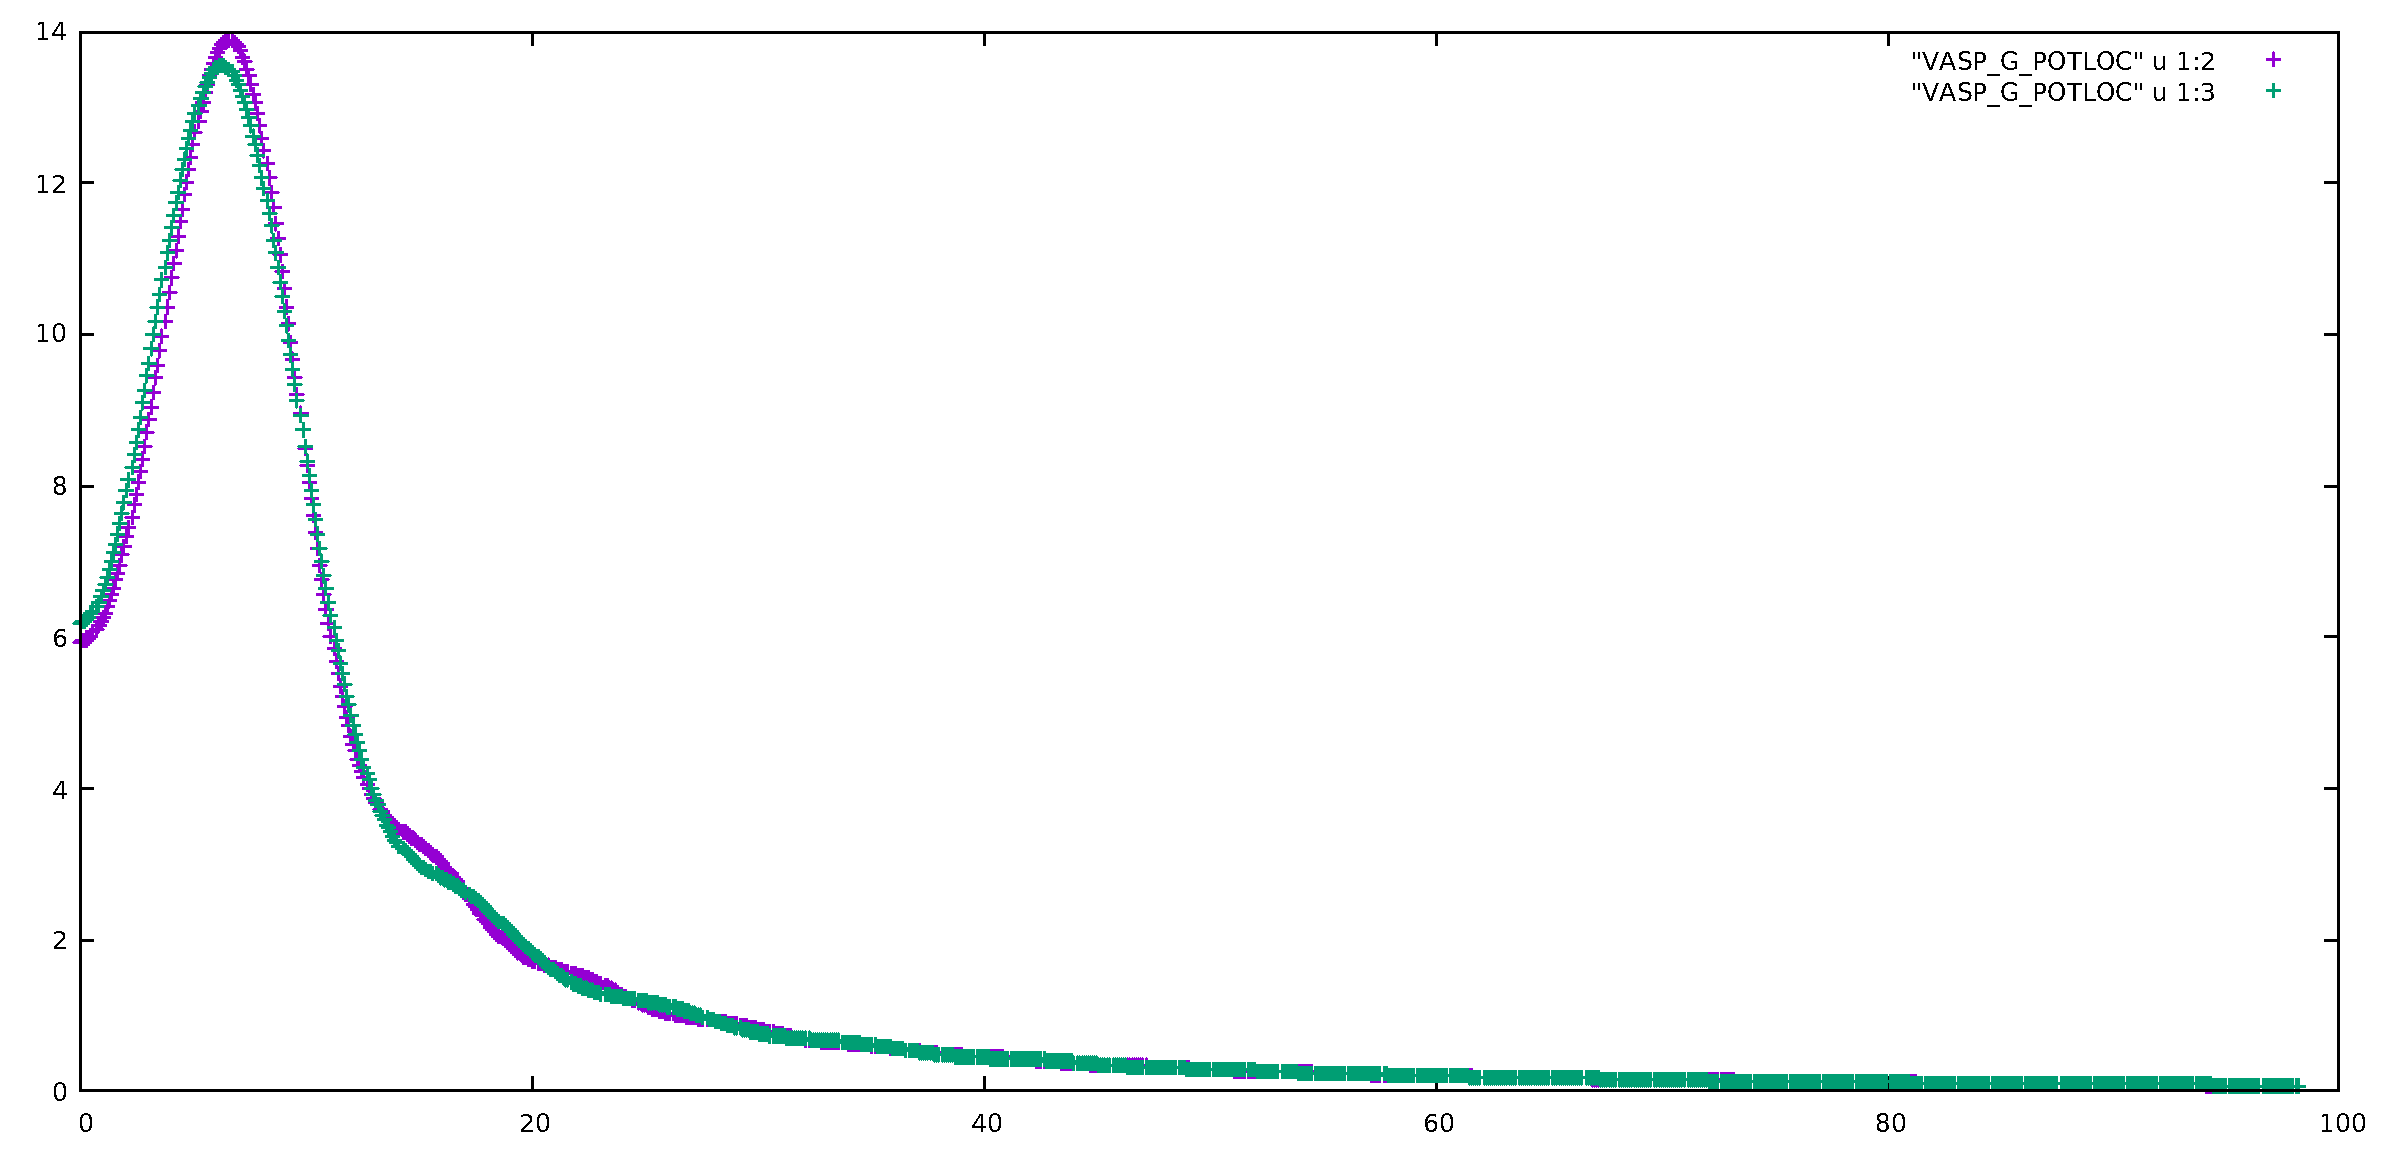
\includegraphics[width=2.3in,height=1.75in,viewport=0 0 1150 650, clip]{Figures/POT_G-dat.pdf}
\vskip -2pt
\caption{\tiny \textrm{The pseudo local ionic pseudo-potential in reciprocal space.}}%(与文献\cite{EPJB33-47_2003}图1对比)
\label{local-potential}
\end{figure}
}

\section{机器学习方法提升参数优化}
\frame
{
	\frametitle{赝化函数的参数优化}
\begin{figure}[h!]
\vspace*{-0.15in}
\centering
%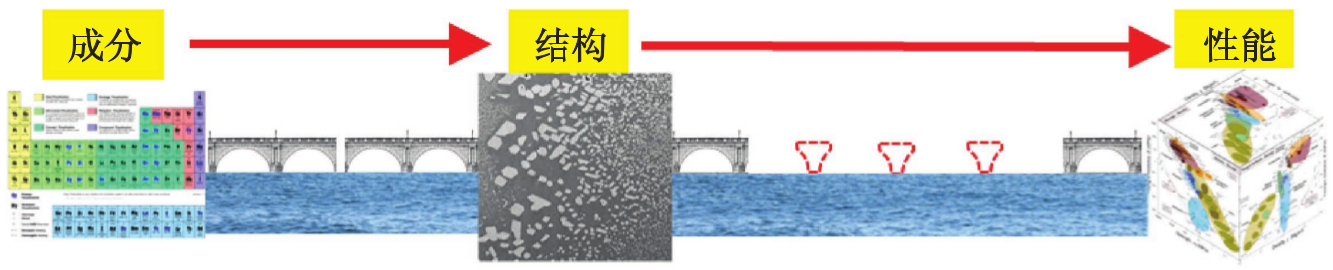
\includegraphics[height=0.60in,width=3.05in]{Figures/MGE-2.png}
%\caption{\tiny \textrm{Pseudopotential for metallic sodium, based on the empty core model and screened by the Thomas-Fermi dielectric function.}}%(与文献\cite{EPJB33-47_2003}图1对比)
%\vskip 0.05pt
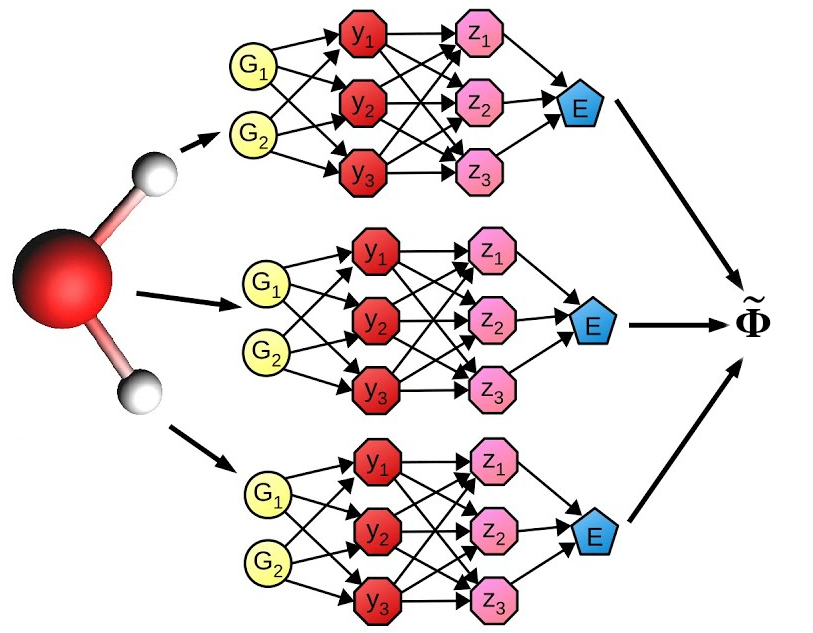
\includegraphics[height=2.50in,width=3.40in]{Figures/Pseudowave_GNN.png}
%\caption{\tiny \textrm{Pseudopotential for metallic sodium, based on the empty core model and screened by the Thomas-Fermi dielectric function.}}%(与文献\cite{EPJB33-47_2003}图1对比)
\label{MLP-GNN}
\end{figure}
基于\textrm{DNN}，无需更多的物理知识，引入更多的可调控参数，逼近精确的赝波函数$\tilde\phi_i(\varepsilon^l_i, r_i,a,b,c)$或赝势函数
}

\frame
{
	\frametitle{\textrm{DNN}优化的赝分波函数}
分波赝波函数的构建:~2层神经网络
\begin{figure}[h!]
\centering
\vskip -0.15in
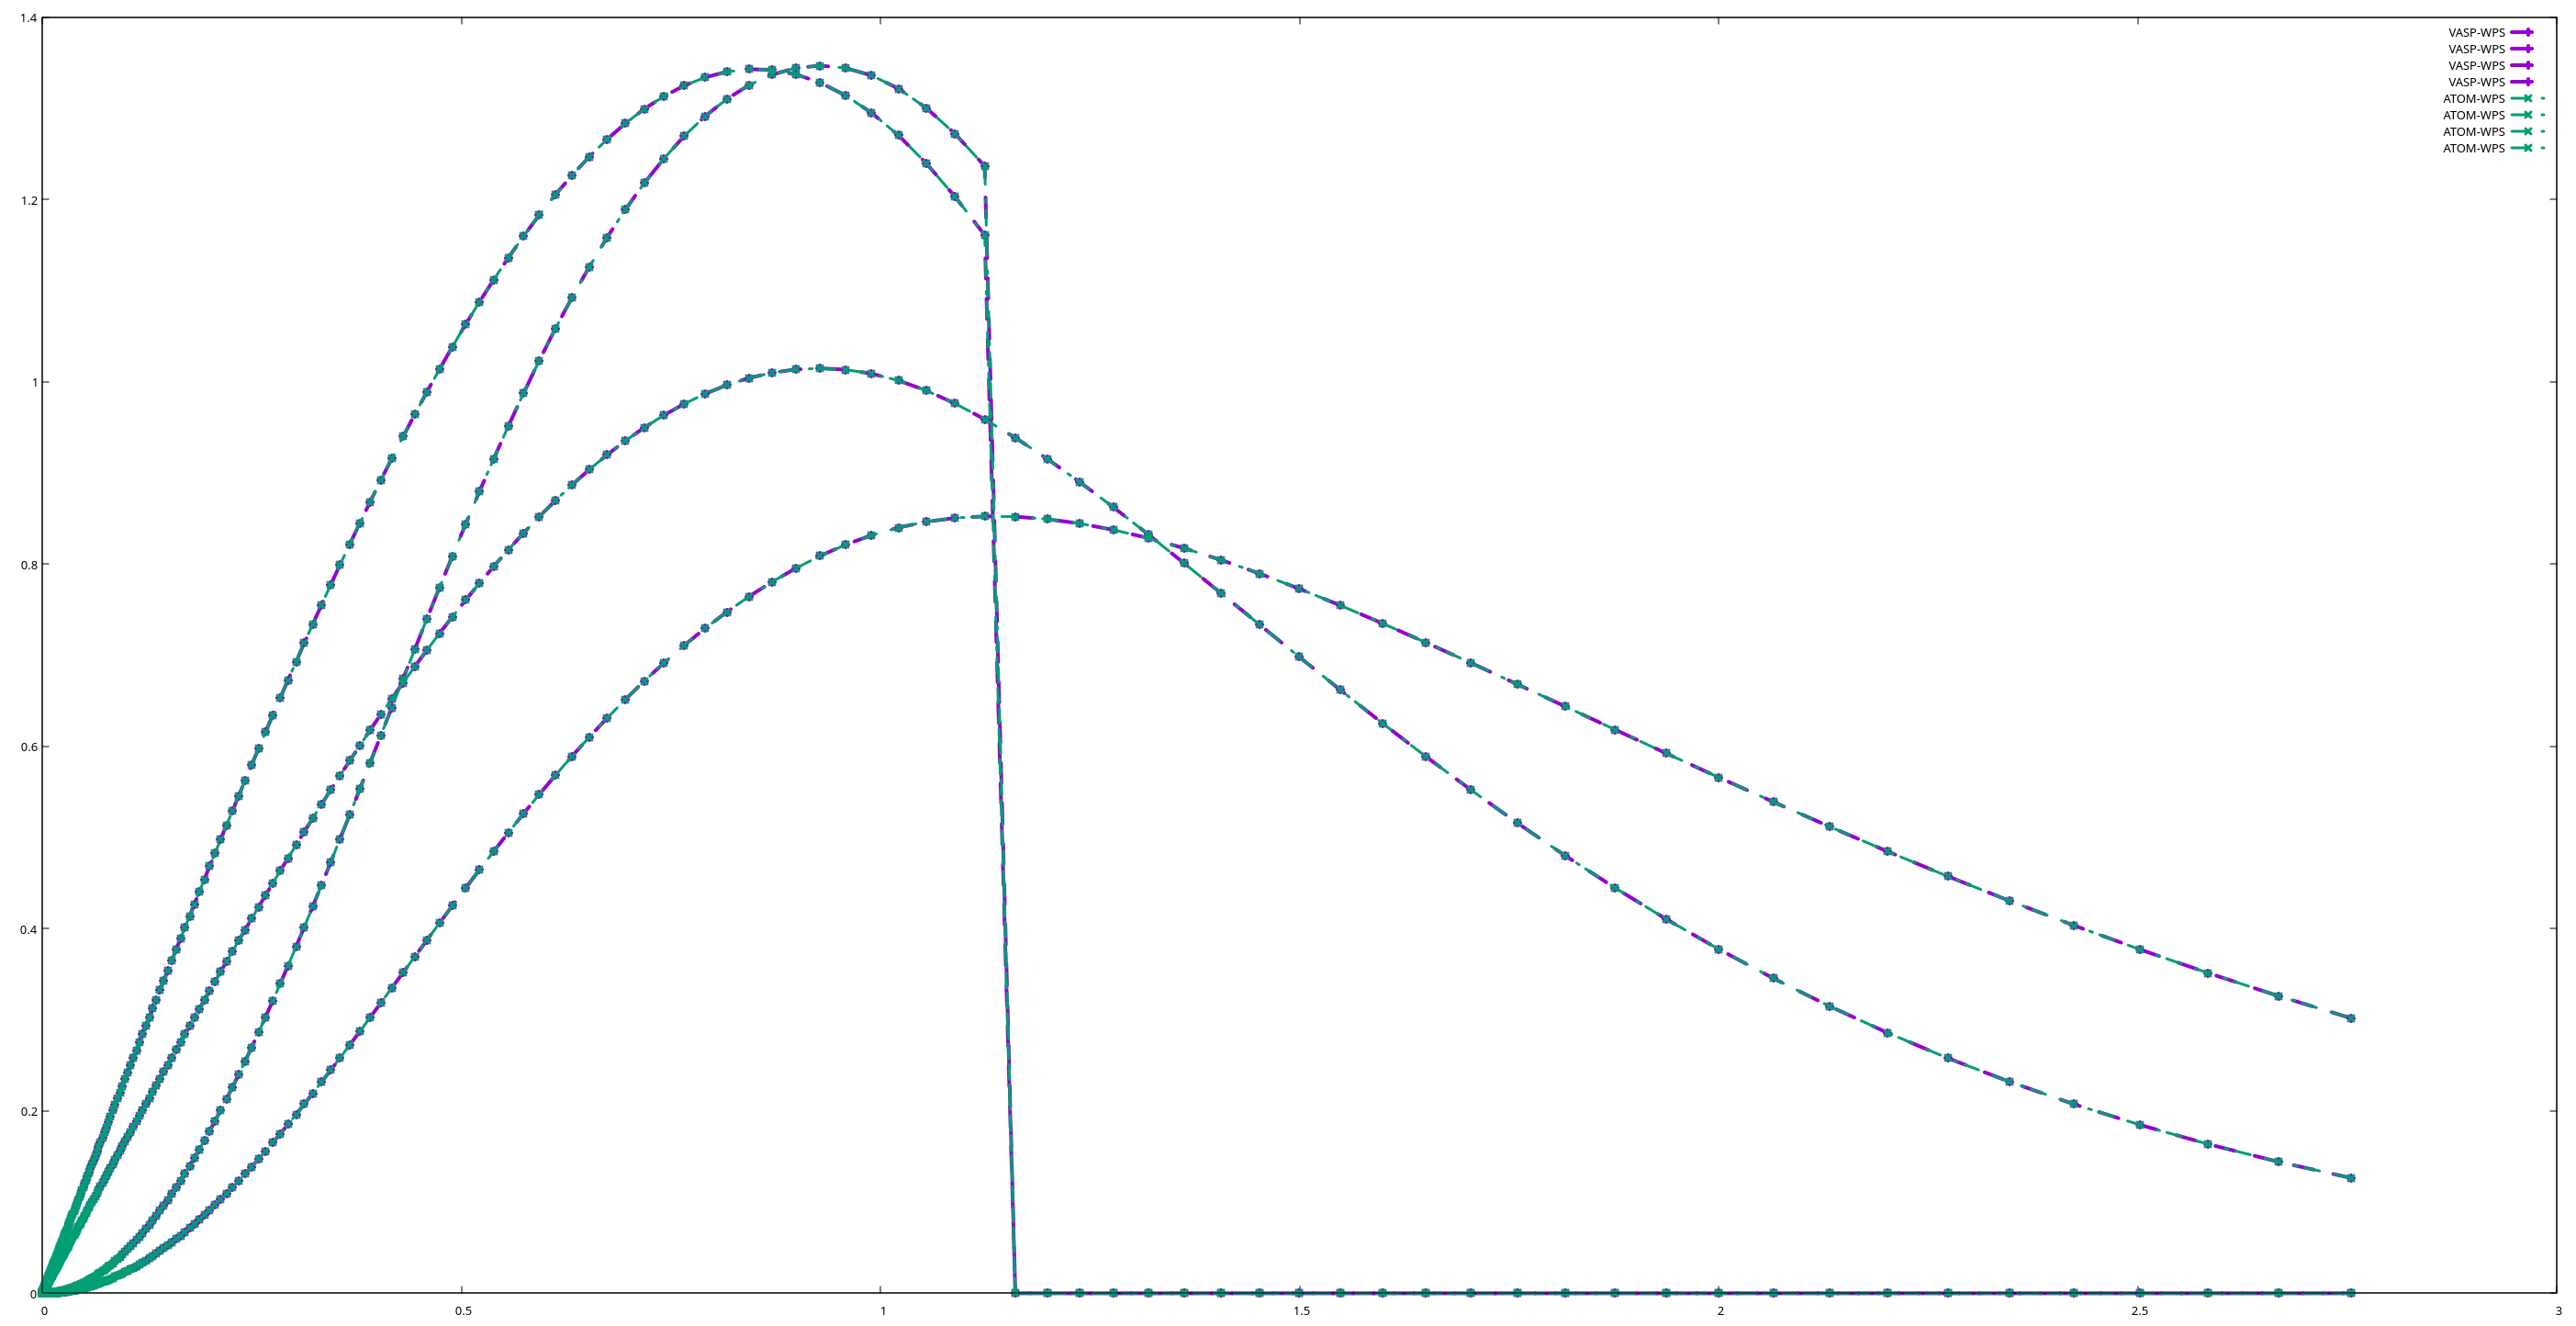
\includegraphics[width=3.6in,height=2.3in,viewport=0 0 2156 1144, clip]{Figures/WPS-data-GNN.png}
\caption{\tiny \textrm{The partial wave function from DNN.}}%(与文献\cite{EPJB33-47_2003}图1对比)
\label{Wave_Function-GNN}
\end{figure}
}

\frame
{
	\frametitle{\textrm{DNN}优化的倒空间局域赝势函数}
局域赝势函数的到空间表示:~5层神经网络
\begin{figure}[h!]
\centering
\vskip -0.15in
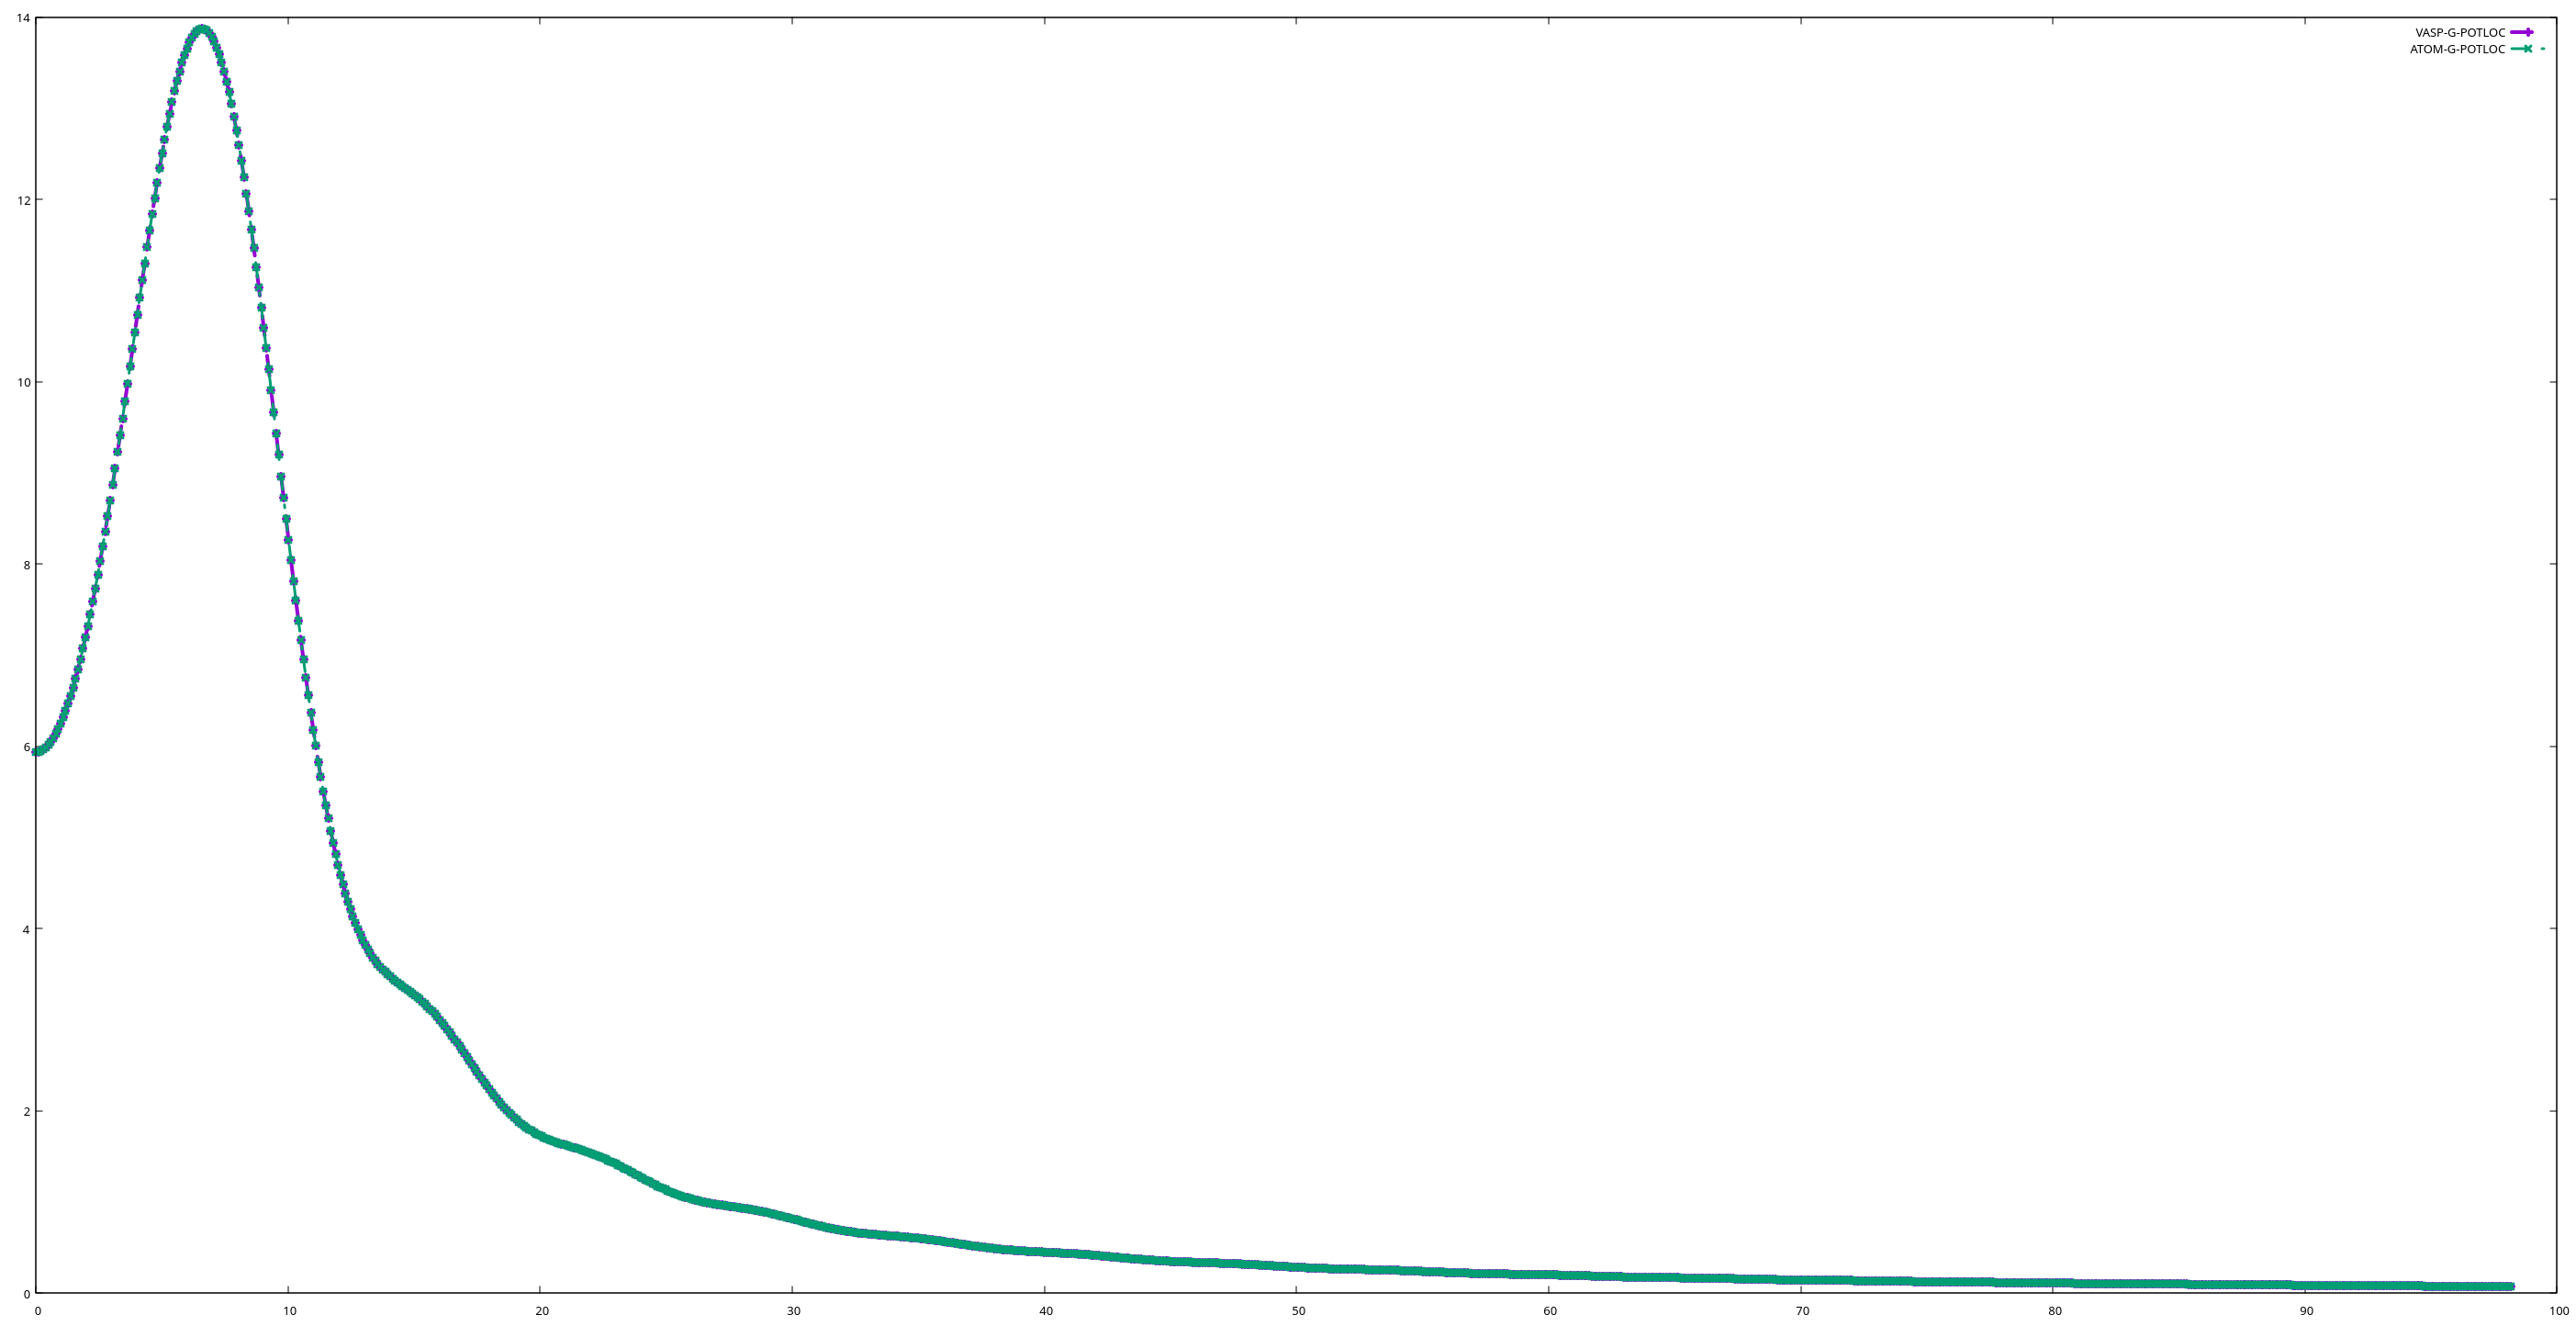
\includegraphics[width=3.6in,height=2.3in,viewport=0 0 2156 1144, clip]{Figures/POTGLOC-data-GNN.png}
\caption{\tiny \textrm{The psedudo local potential function in reciprocal space from DNN.}}%(与文献\cite{EPJB33-47_2003}图1对比)
\label{POT-G-LOC-GNN}
\end{figure}
}

\frame
{
	\frametitle{\textcolor{red}{失败}:~\textrm{DNN}优化的投影函数}
	\textrm{DNN}对初始解析函数的显著依赖
\begin{figure}[h!]
\centering
\vskip -0.15in
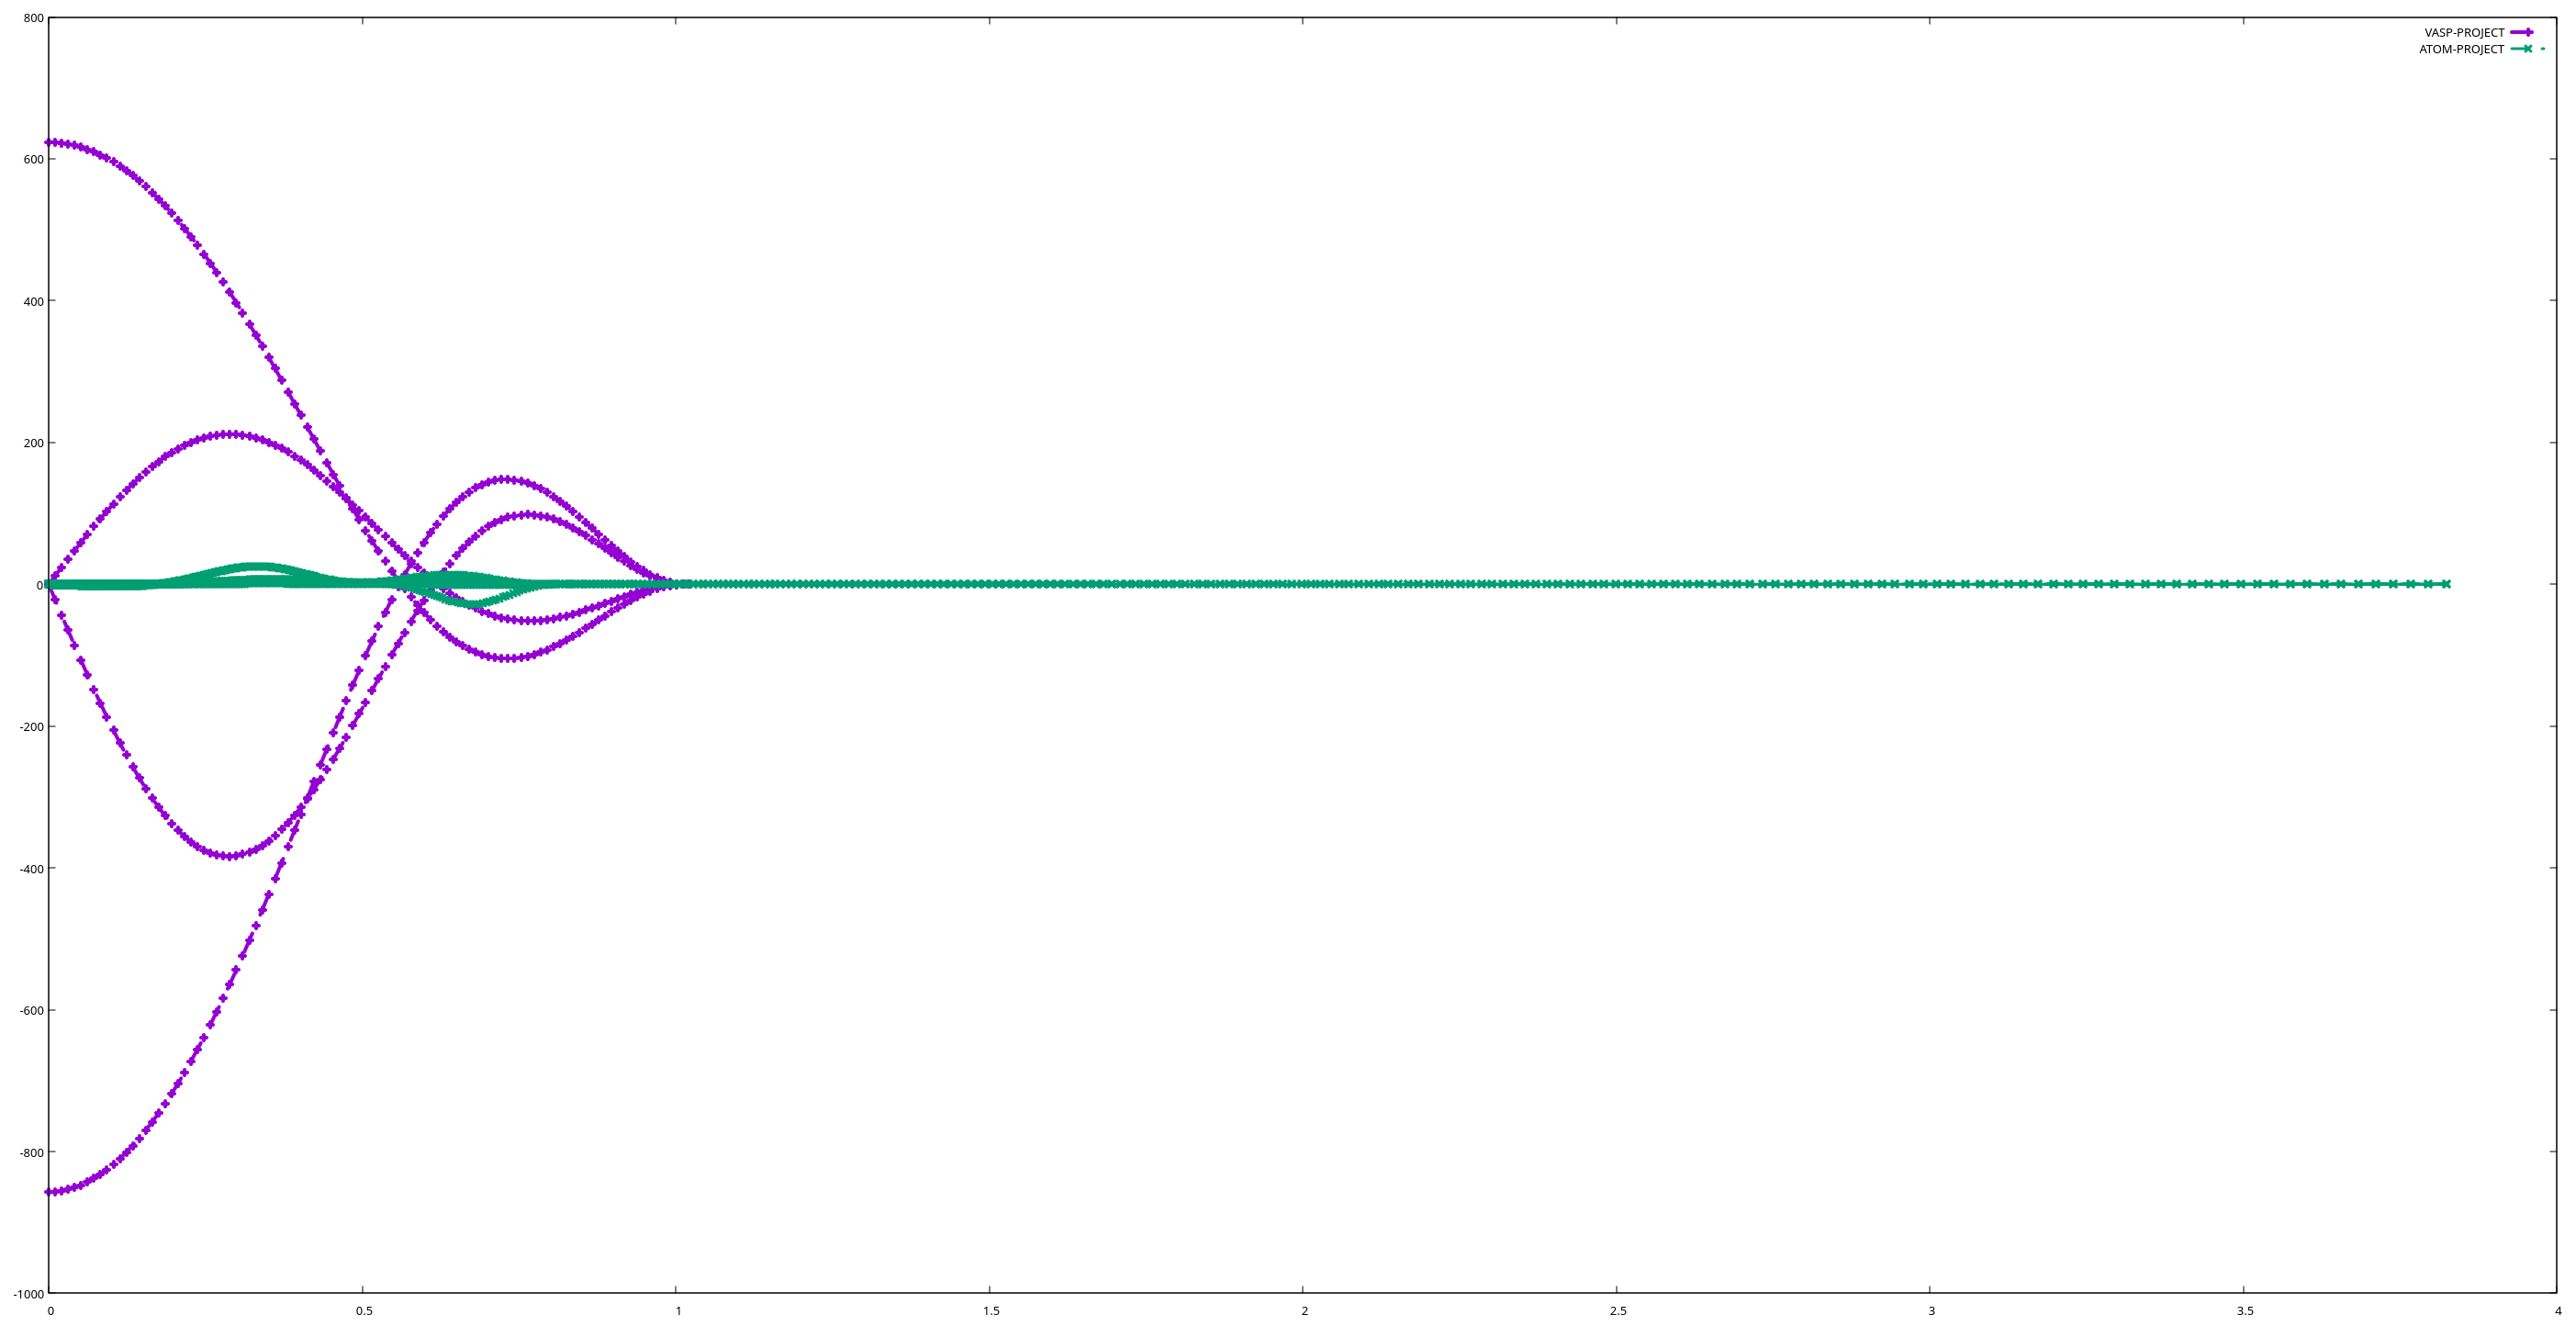
\includegraphics[width=3.6in,height=2.3in,viewport=0 0 2156 1144, clip]{Figures/PROJECT-data.png}
\caption{\tiny \textrm{The project function from vasp and from Atompaw.}}%(与文献\cite{EPJB33-47_2003}图1对比)
\label{PROJECT}
\end{figure}
}

\frame
{
	\frametitle{小结:~机器学习构建\textrm{POTCAR}文件}
	\textrm{DNN}方法构造原子数据集的优势:
	\begin{itemize}
		\item 克服了原有基于物理参数生成\textrm{POTCAR}数据的解析型函数的调控困难\\
			{\fontsize{8.0pt}{5.2pt}\selectfont{\textcolor{magenta}{多参数调控的难度大大降低}}}
		\item 提升了开源软件的产生更精准原子数据的能力\\%，扩展\textrm{PAW}方法的应用场景的条件初步具备\\
			{\fontsize{8.0pt}{5.2pt}\selectfont{\textcolor{magenta}{通过增加径向布点，获取更多近核的波函数信息\\
			为\textrm{ABINIT}、\textrm{QE}提供更合理的原子数据}}}
%		\item 多层神经网络为产生数据更丰富的\textrm{POTCAR}提供了可能\\
%			\textcolor{magenta}{现有\textrm{POTCAR}数据主要包括波函数、电荷密度和势函数信息，磁性}
	\end{itemize}
%}
%
%\frame
%{
%	\frametitle{小结:~机器学习构建\textrm{POTCAR}文件}
	该方法的不足:
	\begin{itemize}
		\item 原有参数的物理信息缺失\\
			{\fontsize{8.0pt}{5.2pt}\selectfont{\textcolor{blue}{参数本身的复杂度增加，参数的物理含义变得模糊}}}
		\item 投影函数的构造\\
			{\fontsize{8.0pt}{5.2pt}\selectfont{\textcolor{blue}{当初始解析函数不够理想，\textrm{DNN}也无法弥补}}}
		\item 对原始\textrm{POTCAR}数据的依赖还没有完全脱离\\
			{\fontsize{8.0pt}{5.2pt}\selectfont{\textcolor{blue}{数据的可靠性验证，还依赖\textrm{POTCAR}数据}}}
	\end{itemize}
极端条件模拟的\textrm{POTCAR}生成方案，还有待合理的检验数据
}

\section{展望:~\rm{AI}技术助力赝势与原子数据的重建}
\frame
{
	\frametitle{应用\rm{AI}技术深化原子数据的认识}
	应用\textrm{AI}技术，投喂足够的\textrm{POTCAR}涵盖的各类型原子数据
	\vskip 5pt
	{\fontsize{14.0pt}{5.2pt}\selectfont{\begin{itemize}
    \setlength{\itemsep}{20pt}
		\item 获得赝分波函数中参数的生成方案，及其对物理含义的理解
		\item 形成可适应更复杂化学环境的\textrm{POTCAR}原子数据
%		\item 系统地\textrm{PAW}原子数据集生成方案
		\item 跨越\textrm{Kresse-PAW}方法\\
\end{itemize}}}
			构建支持赝势-\textrm{PAW}-全势计算的通用\textrm{PAW}原子数据集
}
\appendix
%------------------------------------------------------------------------Reference----------------------------------------------------------------------------------------------
%\begin{thebibliography}{99}
%-----------------------------------------------------------------------------------------------------------------------------------------------------------------------%
%\frame
%{
%\frametitle{主要参考文献}
%{\small
%\bibitem{Singh_Book}\textrm{D. J. Singh. \textit{Plane Wave, PseudoPotential and the LAPW method} (Kluwer Academic, Boston,USA, 1994)}					%
%  \nocite{*}																				%
%}
%}
%\end{thebibliography}

		\frame[allowframebreaks]
		{
\begin{thebibliography}{99}
\frametitle{主要参考文献}
{\tiny
	\bibitem{PRB41-7892_1990}\textrm{D. Vanderbilt. \textit{Phys. Rev.} B, \textbf{41} (1990), 7892} 
	\bibitem{PRB50-17953_1994}\textrm{P. E. Bl\"ochl. \textit{Phys. Rev.} B, \textbf{50} (1994), 17953}
	\bibitem{JPCM6-8245_1994}\textrm{G. Kresse and J. Hafner. J. Phys: \textit{Condens. Matter}, \textbf{6} (1994), 8245}
	\bibitem{PRB59-1758_1999}\textrm{G. Kresse and D. Joubert \textit{Phys. Rev.} B, \textbf{59} (1999), 1758}
	\bibitem{Andersen_Book}\textrm{O. K. Andersen. \textit{Computational Methods in Band Theory} (Plenum, New York, USA, 1971)}
	\bibitem{Nemoshkalenko-Antonov}\textrm{V. V. Nemoshkalenko and V. N. Antonov. \textit{Computational Methods in Solid State Physics} (Gordon and Breach Science Publisher, Amsterdam, The Netherlands, 1998)}
	\bibitem{Elect_Stru}\textrm{Richard. M. Martin. \textit{Electronic Structure: Basic Theory and Practical Methods} (Cambridge University Press, Cambridge, England, 2004)}
}
\end{thebibliography}
\nocite*{}
}
%{\small
%-----------------------------------------------------------Beamer下不建议使用bib,因为涉及分页--------------------------------------------------------------------------%
%{\small
%\phantomsection\addcontentsline{toc}{section}{Bibliography}	 %直接调用\addcontentsline命令可能导致超链指向不准确,一般需要在之前调用一次\phantomsection命令加以修正	%
%\bibliography{Myref}																			%
%\bibliographystyle{mybib}																		%
%  \nocite{*}																				%
%}

%------------------------------------------------------------------------------------------------------------------------------------------------------------------------------%

%-------------------------------------------------------------------------Thanks------------------------------------------------------------------------------------------------
%\section{致谢}
%\frame
%{
%\frametitle{致$\quad$谢}
%\begin{itemize}
%    \setlength{\itemsep}{20pt}
%  \item 感谢本团队高兴誉、吴泉生、宋红州等各位老师参与的讨论
%  \item 感谢莫所长、宋主任以及软件中心各位老师和同事
%  \item 感谢王崇愚先生的帮助
%\end{itemize}
%}
%-------------------------------------------------------------------------------------------------------------------------------------------------------------------------------
